	% This is based on the LLNCS.DEM the demonstration file of
% the LaTeX macro package from Springer-Verlag
% for Lecture Notes in Computer Science,
% version 2.4 for LaTeX2e as of 16. April 2010
%
% See http://www.springer.com/computer/lncs/lncs+authors?SGWID=0-40209-0-0-0
% for the full guidelines.
%
\documentclass{llncs}
\usepackage{graphicx}
\usepackage{tabulary}
%\usepackage{tikz}
\usepackage{pgfplots}
\usepackage[simplified]{pgf-umlcd}
\usepackage{listings}
\usepackage{array}
\usepackage[left=1.2cm,right=1.2cm,top=2cm,bottom=2cm]{geometry}
\graphicspath{ {images/} }
\lstdefinestyle{customhtml}{
  language=HTML,
  showstringspaces=false,
  basicstyle=\scriptsize\ttfamily,
  keywordstyle=\bfseries\color{green!40!black},
  commentstyle=\itshape\color{purple!40!black},
  identifierstyle=\color{blue},
  stringstyle=\color{orange},
  tabsize=2
}

\definecolor{javared}{rgb}{0.6,0,0} % for strings
\definecolor{javagreen}{rgb}{0.25,0.5,0.35} % comments
\definecolor{javapurple}{rgb}{0.5,0,0.35} % keywords
\definecolor{javadocblue}{rgb}{0.25,0.35,0.75} % javadoc
\definecolor{javaStringBlue}{rgb}{0.1647,0,1}

\lstdefinestyle{customjava}{
language=Java,
basicstyle=\footnotesize\ttfamily,
keywordstyle=\color{javapurple}\bfseries,
stringstyle=\color{javaStringBlue},
commentstyle=\color{javagreen},
morecomment=[s][\color{javadocblue}]{/**}{*/},
tabsize=4,
showspaces=false,
showstringspaces=false
}

\linespread{0.97}
\renewcommand{\baselinestretch}{0.89}

\begin{document}

\title{Collaborative Platform for Analysis of Software Systems}
%
\titlerunning{Collaborative Platform}  % abbreviated title (for running head)
%                                     also used for the TOC unless
%                                     \toctitle is used
%
\author{Catarina Isabel Carvalho Santana}
%
\authorrunning{Catarina Santana} % abbreviated author list (for running head)
%
%%%% list of authors for the TOC (use if author list has to be modified)
\tocauthor{Catarina Santana}
%
\institute{Instituto Superior T\'{e}cnico,\\
\email{catarina.santana@tecnico.ulisboa.pt}}
% * <catarinasantana_3@hotmail.com> 2014-12-11T16:24:19.200Z:
%
%  kandlksrn
%

\maketitle              % typeset the title of the contribution

\begin{abstract}
The Software Architectures course at Instituto Superior T\'{e}cnico teaches students the most important concepts on design and architecture of software systems and helps students to apply these concepts to real and complex software systems. Organizing knowledge and applying theory to practice is not an easy task, and students often need to ask questions and discuss. State-of-the-art on collaborative, social software and knowledge structuring was analyzed and a social platform was developed to help solving these problems.

\keywords{social software, knowledge structuring, collaborative platform, reputation systems, tagging systems, ontology, taxonomy}
\end{abstract}
%
\section{Introduction}
\label{introduction}
Analyzing and discussing big, real, open-source and highly complex software system is a very important part of the Software Architectures course at Instituto Superior T\'{e}cnico. In the course context, students must apply concepts and techniques for design and analysis of software architectures to descriptions of real systems. However, applying these concepts and techniques is not a very easy task, and often students have questions and doubts regarding these descriptions. These questions sometimes require not only consulting the course bibliography, but also discussing with peers or asking questions to teachers. This thesis focuses on providing a solution for this problem with the use of social software and knowledge structuring strategies.

This document is organized as follows: Section \ref{problemDescription} gives a more detailed description about the problem of applying theoretical concepts to practical examples in the context of the Software Architectures course. Section \ref{objectives} elicits the main goals of this thesis. Section \ref{relatedWork} presents the state-of-the-art in the areas of Social Software and Knowledge Structuring. Section \ref{solution} gives a small description of the developed solution. Sections \ref{domainModel}, \ref{architecture} and \ref{implementation} describe the solution domain model, architectural details and implementation. Finally, Section \ref{evaluation} will show the assessment of the developed solution and \ref{futureWork} will describe what can still be added to it.

\section{Problem Description}
\label{problemDescription}
The course of Software Architectures teaches students the most important concepts in the field of software architectures and applies these concepts to real-life software systems.

The practical component of this course (where the theory is applied) is done by analyzing documents/articles that describe the architectures of real-life systems and applying the concepts learned in theory lessons: extracting stakeholders, scenarios, tactics, views, etc.
This analysis is either done by students with the help of the teacher, during practical classes, or in work groups where they read, discuss and analyze software descriptions together and present their results to both the teacher and the rest of the class.

Understanding the analysis done and how it was done is very important, since it means students can apply the concepts learned not only in the written exam to pass the course, but also in the future, in other real-life software systems.
However, there are several issues regarding the application of theory concepts in this course:
\begin{itemize}
\item Each year, there are around one-hundred students signed in the course. All these students have roughly the same Computer Science background knowledge. However, not all students have the same maturity: while some may quickly understand what is taught in theory lessons, others may need some more time to assimilate what was taught.

\item The output of the analysis done to software descriptions (the scenarios, etc. extracted) is not available in a consistent way: the analysis done in class is available for students if they took their own notes, and the analysis done by groups is available if students took notes of their colleagues' presentations or groups share their presentation slides among them. Slides may include errors pointed out by the teacher, but not corrected.

\item The case description is usually a fairly long document (from ten to twenty pages approximately). The task of carefully reading and understanding all the text and do a mapping between the concrete descriptions in the text and the abstract concepts learned in theory classes is not easy, as the parts of the text that map to concepts are not always evident.

\item The architectural elements extracted from a single software description are usually scattered along the whole text, and it is not evident the connection between all the elements.

\end{itemize}

\section{Objectives}
\label{objectives}
To solve the problems mentioned in Section \ref{problemdescription}, a collaborative platform was planned and developed, where students and teachers collaborate in the analysis and synthesis of the case descriptions, ending on a structured representation of the case descriptions, that is hooked on the concrete description. 

The goal of the platform is to provide ways for annotating the text on the case descriptions, which will help students organizing their thoughts and creating the structure, and use elements of social software, as a way of promoting collaboration, mutual aid, learning and even some competition between students.
 
The existence of this collaborative should provide not only a way for students to discuss, ask questions and consolidate their knowledge, but also a unique place where their study materials are stored and organized, facilitating their studies.

\section{Related Work}
\label{relatedWork}
The platform to develop can be thought of a social software, where different people communicate and collaborate to provide a structured representation of a software description.
The next sections provide an overview on the state-of-the-art of two main aspects:
\begin{itemize}
\item \textbf{Collaborative work}, presenting the state-of-the-art on social and collaborative aspects of software. This includes literature on the \textbf{Honeycomb Framework}, a framework that generalizes the most important components of social software, \textbf{Persuasive Software}, systems that have impact on users behavior and thoughts, which is the case of the platform to develop, \textbf{Roles in Social Networks}, describing the types of users of social software and \textbf{Reputation Systems}, which is the attribution of scores to users to provide a motivational component on the platform.
	
\item \textbf{Knowledge Structuring}, presenting the state-of-the-art on ways of structuring information. This includes literature on \textbf{Collaborative tagging }systems, which consists of assigning keywords to documents or parts of documents, \textbf{Semi-structured content}, which consists of providing a way for structuring knowledge without such strict rules as, for example, an ontology or a taxonomy and \textbf{Ontology Learning}, extracting knowledge from text.
\end{itemize}

\subsection{Honeycomb Framework}
The definition of Social Software as ``systems that allow people, in their particularities and diversity, to communicate (interact, collaborate, exchange ideas and information) mediating and facilitating any kind of social relationship and favoring the emergence of a collective wisdom and a bottom-up organization'' \cite{pereira2010social} applies to our collaborative platform, as it should allow students with different personalities and opinions to participate by identifying architectural elements, asking questions, etc. in order to reach a complete and correct analysis of that system. 

The Honeycomb Framework was proposed to illustrate the seven elements that give a functional definition for social software \cite{smith2007social}: \textbf{Identity}, the unique identifier of a user within the system, which applies to the platform to develop in the sense that each student is a unique person and must have a unique identification in the platform; \textbf{Presence}, resources that allow knowing if certain identity is online, which are not strictly necessary in the platform; \textbf{Relationship}, way to determine how users can relate/are related to others, which applies to the platform as students are related to each other both as colleagues as and group elements, and to the teachers; \textbf{Reputation}, way of knowing the status of a user in the system, which could be used to assess the quality and relevance of the contributions to the platform; \textbf{Groups}, possibility to form communities of users that have common interests, which applies to the platform as students form work groups; \textbf{Conversation}, resources for communication among the users (synchronous and/or asynchronous). In the context of the platform, conversation should be done asynchronously with comments and discussions; \textbf{Sharing}, possibility of sharing objects that are important to the users (videos, images, etc), which applies to this context as students may want to share documentation or other media with their colleagues or their group;

\subsection{Persuasive Software Design Patterns}
The term ``persuasive technology'' is used to describe computer systems that have an impact on user's thoughts and may even lead to changes in their behavior \cite{fogg2002persuasive,oinas2009persuasive}.

There are three different possible outcomes for a persuasive system: \textbf{Reinforcement}, making current attitudes resistant to change, \textbf{Changing Outcome }, changes in a person's response to an issue, and \textbf{Shaping Outcome}, formulate a pattern for a situation where one did not exist before \cite{oinas2008towards}. The most important outcome for this platform is the Changing Outcome: When a description of a system is presented, the students most not only read it, but also relate it to the concepts learned and use the platform to try and extract the correct scenarios and views from it.

The concept of social influence describes a change in one's behavior (or attitudes or beliefs), caused by external pressures \cite{guadagno2010preference}. In our context, students may not contribute to the platform at first, but may feel compelled to when seeing their colleagues' contributions. Four design patterns are proposed for persuasive systems, in order to introduce social influence in software features: Social Learning and Facilitation (SLF), Competition (COM), Cooperation (COO) and Recognition (REC) \cite{oduor2014persuasive}. 

The \textbf{Social Learning and Facilitation} pattern has the main purpose of using software features that allow to visualize the presence of other people, with the motivation that it is easier for individuals to pursue their goals if there is a clear awareness of other people pursuing the same goal and facing the same issues \cite{oduor2014persuasive}. In the context of our collaborative platform, students may not contribute at first, but may feel compelled to as they see their colleagues contributing.

The \textbf{Competition} pattern has the main purpose of using competitive elements, such as ranks, scores and levels, that allow users to compare their performance with others, and adjust their target goals based on these. Some people may see this competition as a source of anxiety, so participation must be voluntary \cite{oduor2014persuasive}. Adding a score for each student and a rank hierarchy based on the range of scores will start a hopefully healthy competition between them. Anonymity should be an option in the platform, to remove sources of anxiety.

The \textbf{Cooperation} pattern has the main purpose of providing software features that allow users to engage in mutual goals and support each other. The motivation for this pattern is that it is easier to cooperate if people are engaged in mutual objectives. However, some people prefer to perform alone, so cooperation must not be forced \cite{oduor2014persuasive}. The students in the platform will be working towards a main goal: correctly understanding and correlating what was learned in the Software Architectures classes with real examples of software systems. But there are several concepts and structures to identify on a single description and students may have difficulties in identifying them, so dividing the main goal in several smaller goals and have discussions around them would be useful.

The \textbf{Recognition} pattern has the purpose of providing software features that enable users to get recognition from their peers. The motivation for this pattern is that users sometimes need a reason to focus on reaching their goals. Having their efforts recognized may be a good reason to keep the good work\cite{oduor2014persuasive}. As the system should have a score system, it could be used as a way of creating a weekly top ten of the students who achieved most points in that week. Recognition is then achieved when students see their names highlighted.

\subsection{Roles in Social Networks}
A \textit{role}, in a social structure, is a set of expectations for an individual in a certain position. For example, the role of ``secretary'' is associated to what secretaries are expected to do \cite{forestier2012roles,nadel1957theory}. There are two categories of roles: \textit{Non-explicit roles}, which are not defined a-priori but can be inferred, and \textit{Explicit roles}, which are predefined types of actors in the social network, such as ``experts'' or ``influencers''.

In the platform to develop, it is possible to define a priori the two main roles: the \textbf{Students}, which are the most active users in the platform as they contribute to the analysis of the software descriptions, and the \textbf{Teachers} which corresponds to a very small number of users in the platform. Their number of contributions is smaller and they are mostly for adding correction to the contents added by the students to the platform.

\subsection{Reputation Systems}
\label{repsys}
Reputation systems are of extreme importance for certain kinds of applications, namely e-commerce websites, where money transactions are executed and the reputation of a seller will denote the degree of trust that possible buyers will have in them \cite{vavilis2014reference}.

For the platform to develop, reputation does not play such an important role, but will add a motivational component to the platform: Students rate their colleagues' contributions and should try to get and keep a high reputation score. The motivation behind the importance of including a reputation system in the platform is the study conducted \cite{dencheva2011dynamic}, concerning the lack of participation in Moknowpedia, a Wiki system. A reputation system was added to the wiki in order to solve these problems and improve both content quality and quantity\cite{prause2008approach}, and results showed an increase of 62\% in the number of article revisions and an increase of 42\% in the number of viewed articles.
	
\subsubsection{Requirements and Features of the Reputation System:}

A framework for analysis of reputation systems is proposed in \cite{vavilis2014reference}, where the general requirements for reputation systems are elicited and the corresponding features needed for their fulfillment. Given the context of the platform, its reputation system requires that \textbf{Ratings and Reputation should discriminate user behavior}, as these scores should allow to identify students with few and/or less relevant contributions and students with many and/or very relevant ones, \textbf{the reputation system should be able to discriminate ``incorrect'' ratings}, as malicious users are present everywhere and can give intentionally inaccurate ratings, \textbf{Users should not be able to modify ratings, reputation values and calculate their own reputation}, as this data should not be accessible to them, and the score should be calculated by the reputation system.

To satisfy the identified requirements, the reputation system should feature a range of values to represent \textbf{trust and distrust}, where low values indicate students with few and/or less relevant contributions and high values indicate students with many and/or very relevant ones, \textbf{absolute reputation values}, calculated independently for each user, and identification of \textbf{origin and target} of the ratings, to prevent self-ratings and identify potential malicious users

\subsubsection{Components of a Reputation System:}
Reputation systems are divided in four components\cite{liu2012systematic,liu2010evaluation}, and each have a set of defined criteria for their evalutation: \textbf{Input}, the process of collecting reputation information from information sources, \textbf{Processing}, the procedure of computing and aggregating the reputation information, \textbf{Output}, the dissemination of the reputation information and the \textbf{Feedback Loop}, the collection of feedback of the output (review of the review), which does not apply to the context of the platform.

Concerning the \textbf{Input} component, ratings are collected in the platform and are given by the students that are logged in. Only a single property is collected, the rating assigned.Concerning the \textbf{Processing} component, a weighted average algorithm is the best choice to aggregate ratings in this simple system, and information should be updated as soon as the ratings are assigned. Both the algorithm and the system have a very low complexity. Concerning the \textbf{Output} component, the end users of the information are the students registered in the platform, and this information is only available inside the platform. The reputation information consists in the result of the weighted average algorithm.

\subsection{Collaborative Tagging}
Collaborative tagging is the practice of allowing anyone to freely attach keywords or tags to content \cite{golder2006usage}. Tagging-based systems contrast with taxonomies as they are neither exclusive nor hierarchical, and allow to identify content as being about a great variety of things simultaneously \cite{golder2006usage}. The tags added to content may describe the content itself, or describe the category in which the content falls \cite{coates2005two}. It is possible to identify several functions for the tags, within the system that uses the tagging system \cite{golder2006usage}.

In this platform we are aiming for using tags from a closed taxonomy as a way of identifying the main parts of a software system within a software description, namely stakeholders, scenarios and their parts, tactics, etc., and use the tagged text to create a structured description of the document.

\subsection{Semi-Structured Content}
Knowledge can be obtained from many different resources, ranging from unstructured (for example, language models obtained from plain text) to structured ones (for example, ontologies) \cite{hovy2013collaboratively}. However, unstructured resources do not allow for complex inference chains\cite{domingos2007toward} and information is not ontologized\cite{hovy2013collaboratively}, and structured resources require a huge amount of effort to create and maintain\cite{hovy2013collaboratively}. Semi-structured contents try to create a middle-ground between these two types. The most important example of their use is the Wikipedia, which is a repository of webpages, related with each other by links. Massive online collaboration allow for updated high quality and wide coverage of contents. To sum up, using semi-structured resources provides the best of both worlds: high quality information with wide coverage of almost all domains \cite{hovy2013collaboratively}.
 
The main goal of this platform is to allow students to extract a semi-structured representation of a software system from a description in plain text, and have all the parts that constitute a software system described in a structure similar to a Wikipedia, instead of scattered along a ten or more pages article. This will be accomplished by creating templates for the concepts and associating information from the document to them. Student collaboration in the platform will lead to good quality structured descriptions of the articles.
	
\subsection{Ontology Learning}
Research on Ontology learning from text has evolved over the years and there are several open challenges for this field \cite{wong2012ontology}. Ontologies are defined as ``effectively formal and explicit specifications in the form of concepts and relations of shared conceptualizations'' \cite{gruber1993translation}, and can be thought of as a directed graph, with concepts as nodes and relations as edges. Techniques for ontology learning can be classified in statistics-based, linguistics-based, logic-based or hybrid.

Regarding the context of the platform, all the concepts used to tag the document contents (the concepts of Software Architectures) and their will be defined a priori. Software description documents do not contain these concepts, but the students' motivation is to find parts of the text that correspond to the concepts predefined and tag them accordingly. This facilitates the comprehension of the text contents and the creation of the semi-structure as mentioned previously.

\section{Solution}
\label{solution}
To solve the problems elicited throughout this document, it was developed a Web Application to be used by students and teachers, both in class and home environments. This kind of application facilitates collaboration between its users, and therefore was the more adequate choice for the system to develop. The developed application features an \textbf{authentication system}, where users can login into the system, \textbf{document management}, only available for teachers, where software description articles can be added or removed, \textbf{document parsing } into a view, creation of \textbf{annotations} in the document text, which are parts of selected text annotated with tags, and \textbf{templates }for a set of Software Architectures concepts, which aggregate the corresponding annotations and describe the concepts.

The next sections will give an overview of the domain, and explain the architecture and implementation of the system.
\section{Domain Model}
\label{domainModel}
To understand the architectural and implementation decisions taken during the solution development, it is necessary to understand the Software Architectures Domain Model. Section \ref{domainModel:SAConcepts} lists and describes the concepts talked in the Software Architectures classes, Section \ref{section:domainModel} presents an abstract domain model where it is possible to see how these concepts relate and Section \ref{section:templates} gives an idea on how the information from the domain model can be represented in templates.

\subsection{Concepts}
\label{domainModel:SAConcepts}
Before describing the domain model of the developed solution, it is necessary to provide a small introduction to the most important concepts from the Software Architectures course.
\subsubsection{Scenarios:}
\label{SAConcepts:Scenarios}
A scenario is used to capture and express the quality requirements of a system. The considered qualities are \textbf{Availability}, \textbf{Interoperability}, \textbf{Modifiability}, \textbf{Performance}, \textbf{Security}, \textbf{Testability} and \textbf{Usability}.

A scenario consists of six parts\cite{bass2003software}: The \textbf{Source of Stimulus}, an entity that generates the stimulus; The \textbf{Stimulus}, a condition that arrives at the system; The \textbf{Environment}, the system condition when the stimulus occurs; The \textbf{Artifact}, the part of the system stimulated; The \textbf{Response}, what is done in response to the stimulus; And the \textbf{Response Measure}, the way of measuring the response. Each Scenario uses a set of \textbf{Tactics}, which are design decisions used to achieve the quality requirements expressed in them. Each quality requirement has a set of commonly used tactics.

\subsubsection{Views:}
\label{SAConcepts:Views}
A view is a representation of a set of system elements and the relationships associated with them \cite{clements2003documenting}. This set of elements and relationships is constrained by viewtypes.
A Viewtype defines the element types and relationship types used to describe the architecture of a software system from a particular perspective. Viewtypes refine into styles, which are specializations of element and relation types, together with a set of constraints on how they can be used.Views can fall into three viewtype categories: 

The \textbf{Module Viewtype}, which documents the system principal units of implementation. The elements are the \textit{Modules} and relationships between them can be of type part-whole, dependency and generalization/specialization; The \textbf{Component \& Connector Viewtype}, which documents the system units of execution. The elements are the Components and the Connectors, and the relationships can be of type \textit{``Attachment''}, associating components to connectors, and \textit{``Interface''} Delegation, associating component ports and connector roles to other ports and roles, respectively; and the \textbf{Allocation Viewtype}, which documents the relationships between a system's software and its development and execution environments. The elements are the \textit{Software Element} (Module, Components and Connector) and the \textit{Environmental Element}. The relationships are of type \textit{``Allocated-to''}, where software element is allocated to an environmental element. 

\subsection{Model}
\label{section:domainModel}
Figure \ref{figure:abstractDomainModel} shows the concepts and relations described in Section \ref{domainModel:SAConcepts} in a Domain Model Diagram.
 
\begin{figure}[ht]
\centering
\renewcommand {\umltextcolor}{black}
\renewcommand {\umlfillcolor}{none}
\renewcommand {\umldrawcolor}{black}

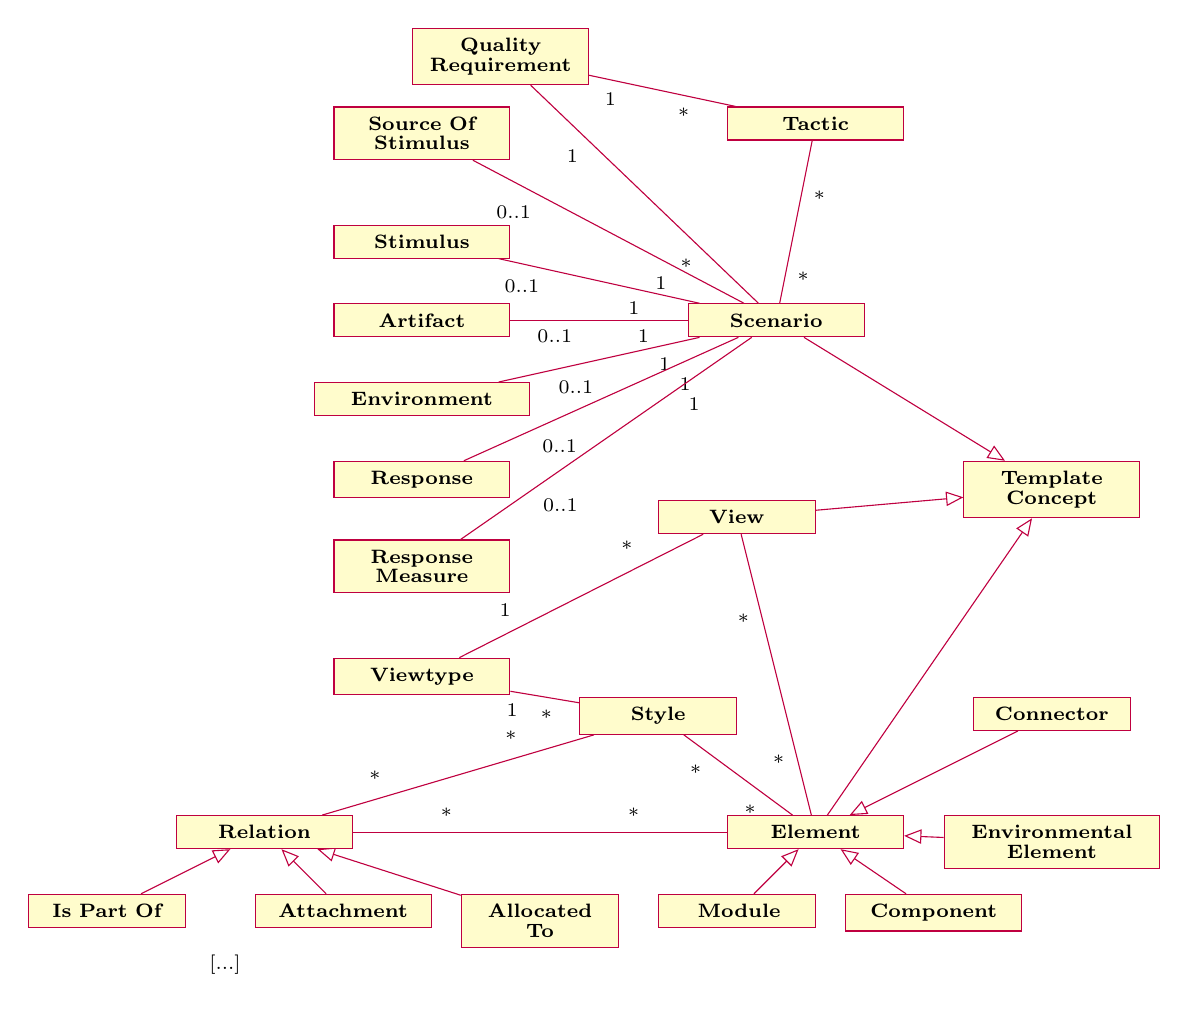
\begin{tikzpicture}
\tikzstyle{every node}=[font=\scriptsize]
\begin{class}[text width=2cm]{Template Concept}{8,-4.5}
\end{class}

\begin{class}[text width=2cm ]{Source Of Stimulus}{0,0}

\end{class}
\begin{class}[text width=2cm ]{Stimulus}{0,-1.5}
%\inherit{ScenarioElement}
\end{class}
\begin{class}[text width=2cm ]{Artifact}{0,-2.5}
%\inherit{ScenarioElement}
\end{class}
\begin{class}[text width=2.5cm ]{Environment}{0,-3.5}
%\inherit{ScenarioElement}
\end{class}
\begin{class}[text width=2cm ]{Response}{0,-4.5}
%\inherit{ScenarioElement}
\end{class}
\begin{class}[text width=2cm ]{Response Measure}{0,-5.5}
\end{class}
\begin{class}[text width=2cm ]{Scenario}{4.5,-2.5}
\inherit{Template Concept}
\end{class}
\begin{class}[text width=2cm ]{Quality Requirement}{1,1}
\end{class}
\begin{class}[text width=2cm ]{Tactic}{5,0}
\end{class}

\begin{class}[text width=1cm ]{View}{4,-5}
\inherit{Template Concept}
\end{class}
\begin{class}[text width=2cm ]{Viewtype}{0,-7}
\end{class}
\begin{class}[text width=1cm ]{Style}{3,-7.5}
\end{class}
\begin{class}[text width=2cm ]{Relation}{-2,-9}
\end{class}

\begin{class}[text width=2cm ]{Element}{5,-9}
\inherit{Template Concept}
\end{class}

\begin{class}[text width=1.5cm]{Is Part Of}{-4,-10}
\inherit{Relation}
\end{class}

\draw [umlcd style] (-2.5,-10.90) node {[...]};

\begin{class}[text width=2cm]{Attachment}{-1,-10}
\inherit{Relation}
\end{class}

\begin{class}[text width=1.5cm]{Allocated To}{1.5,-10}
\inherit{Relation}
\end{class}

\begin{class}[text width=1cm]{Module}{4,-10}
\inherit{Element}
\end{class}

\begin{class}[text width=2cm]{Component}{6.5,-10}
\inherit{Element}
\end{class}

\begin{class}[text width=2.5cm]{Environmental Element}{8,-9}
\inherit{Element}
\end{class}

\begin{class}[text width=1.5cm]{Connector}{8,-7.5}
\inherit{Element}
\end{class}

\association{Source Of Stimulus}{}{0..1}{Scenario}{}{1}
\association{Stimulus}{}{0..1}{Scenario}{}{1}
\association{Artifact}{}{0..1}{Scenario}{}{1}
\association{Environment}{}{0..1}{Scenario}{}{1}
\association{Response}{}{0..1}{Scenario}{}{1}
\association{Response Measure}{}{0..1}{Scenario}{}{1}
\association{Quality Requirement}{}{1}{Scenario}{}{*}
\association{Quality Requirement}{}{1}{Tactic}{}{*}
\association{Scenario}{}{*}{Tactic}{}{*}
\association{View}{}{*}{Viewtype}{}{1}
\association{Viewtype}{}{1}{Style}{}{*}
\association{Style}{}{*}{Element}{}{*}
\association{Style}{}{*}{Relation}{}{*}
\association{View}{}{*}{Element}{}{*}
\association{Element}{}{*}{Relation}{}{*}
\end{tikzpicture}
\caption{Domain Model showing the Software Architectures concepts and how they are related}
\label{figure:abstractDomainModel}
\end{figure}

The scenario elements are associated to the Scenario, and each Scenario captures a single Quality Requirement and has a set of Tactics. A View is associated with a Viewtype, which refines into a style. The View contains a set of elements, which have relations with each other. The Scenario, View and Element are considered the main concepts of the domain, and they have a dedicated template in the developed solution. These templates will contain information about the concept and how it is related with other concepts in the domain model.

\subsection{Templates}
\label{section:templates}
The structured representation of the Software Architectures concepts described in Sections \ref{domainModel:SAConcepts} and \ref{section:domainModel} is represented in the developed solution by using specific templates for these concepts.

It did not make sense to have a template for each and every one of them, as it is easier to see the relations between concepts if they are in the same template. This is the case for the Scenarios. It makes sense to see all the elements of a Scenario together, so it is considered one of the main concepts and has its own dedicated template, in which are present the quality attribute, the elements and the tactics. 

Figure \ref{figure:scenarioTemplate} shows a Schema example for the Scenario template. All the Scenario elements, the quality requirement and the tactics are present in the template, making it possible to see, as mentioned before, how all these concepts are related.

\begin{figure}
\centering
\lstinputlisting[language=HTML, style=customhtml]{scenarioSchema.html}
\caption{Schema for the Scenario template}
\label{figure:scenarioTemplate}
\end{figure}

The Views and their elements are also another case of main concepts. It makes sense to aggregate all the system elements and their relationships from a view in a separate template, representing the part of the system being described in that view. However, since a single element can be present in more than one view, it also makes sense to have a specific template for the elements, so their individual properties can be seen. The templates for the View and View Elements follow the same idea of the Scenario schema. The template for the elements represents the element information and also its relations with other elements. The View template has the particularity that, besides including information about the view, also includes the templates of the elements present in it.

\section{Architecture Analysis}
\label{architecture}
Chapter \ref{domainModel} introduced the domain model of the Software Architectures concepts present in the developed solution, and the templates in which they are included.

In this section, it is shown how these templates are filled with information extracted from a software description article. The next subsections will present two entities from the system: the Document and the Annotation. These entities have a major role in the identification of Software Architectures concepts from the domain model, and the enrichment of the templates for those concepts.

\subsection{Document}
\label{section:document}

The Document entity in this system corresponds to an article which describes a software system and is read and analysed in the practical classes of the Software Architectures course. This entity saves the article text and its source, so it can be parsed locally in the application

Figure \ref{figure:documentEntity} shows the Document entity in the system. The ``title'' attribute corresponds to the title of the article, the ``url'' saves the article's original URL, and the ``content'' saves the article's contents.

\begin{figure}
\centering
\renewcommand {\umltextcolor}{black}
\renewcommand {\umlfillcolor}{none}
\renewcommand {\umldrawcolor}{black}

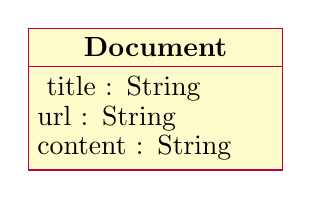
\begin{tikzpicture}
\begin{class}[text width=3cm ]{Document}{0,0}
	\attribute { title : String }
	\attribute { url : String }
	\attribute { content : String }
\end{class}
\end{tikzpicture}
\caption{The Document Entity}
\label{figure:documentEntity}
\end{figure}

As the main purpose of this application is to create a structured representation of the document using the templates described in Section \ref{section:templates}, the instances of the main concepts, from which the templates will be generated, must be associated to the Document, as shown in Figure \ref{figure:documentConcept}. This way, generating a structured representation of the document is as easy as extracting the main concepts that are connected to it and including their respecive templates in the structured representation. A concept describes a part of one and only one document, hence the '1' cardinality.  

\begin{figure}
\centering
\renewcommand {\umltextcolor}{black}
\renewcommand {\umlfillcolor}{none}
\renewcommand {\umldrawcolor}{black}

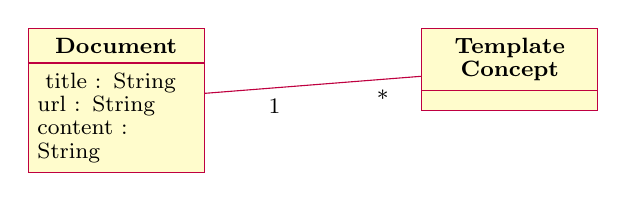
\begin{tikzpicture}
\tikzstyle{every node}=[font=\footnotesize]
\begin{class}[text width=2cm ]{Template Concept}{5,0}
	\attribute{}
\end{class}

\begin{class}[text width=2cm ]{Document}{0,0}
	\attribute { title : String }
	\attribute { url : String }
	\attribute { content : String }
\end{class}

\association{Document}{}{1}{Template Concept}{}{*}
\end{tikzpicture}
\caption{Association between Document and Concept entities}
\label{figure:documentConcept}
\end{figure}

\subsection{Annotation}
\label{section:annotation}

An annotation consists of a portion of text selected from the article, enriched with a tag and other information. This selected text can correspond partially or totally to the specification of a Software Architecture concept. For example, the description of the Source of Stimulus of a Scenario may be found in a single paragraph of the article, or in a set of single sentences scattered along the whole article. 

Figure \ref{figure:annotationEntity} shows the Annotation entity in the system. The ``annotation'' field saves a Json representation of the annotation data such as the quote from the text and the given tag. The ``tag'' field stores the tag given to the annotation. This tag corresponds to a Software Architectures concept, such as ``Stimulus'' or ``Module''.

\begin{figure}
\centering
\renewcommand {\umltextcolor}{black}
\renewcommand {\umlfillcolor}{none}
\renewcommand {\umldrawcolor}{black}

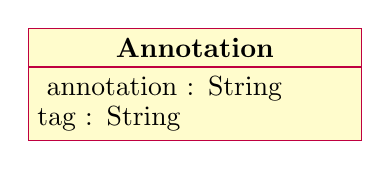
\begin{tikzpicture}
\begin{class}[text width=4cm ]{Annotation}{0,0}
	\attribute { annotation : String }
	\attribute { tag : String }
\end{class}
\end{tikzpicture}
\caption{The Annotation Entity}
\label{figure:annotationEntity}
\end{figure}

Annotations are added to the system by selecting a portion of text in the parsed document and setting it as an annotation. Therefore, an annotation belongs to one, and only one document. In Figure \ref{figure:documentAnnotationConcepts} it is possible to see the association between the Annotation and Document entities, which reflects the mentioned constraints.

\begin{figure}
\centering
\renewcommand {\umltextcolor}{black}
\renewcommand {\umlfillcolor}{none}
\renewcommand {\umldrawcolor}{black}

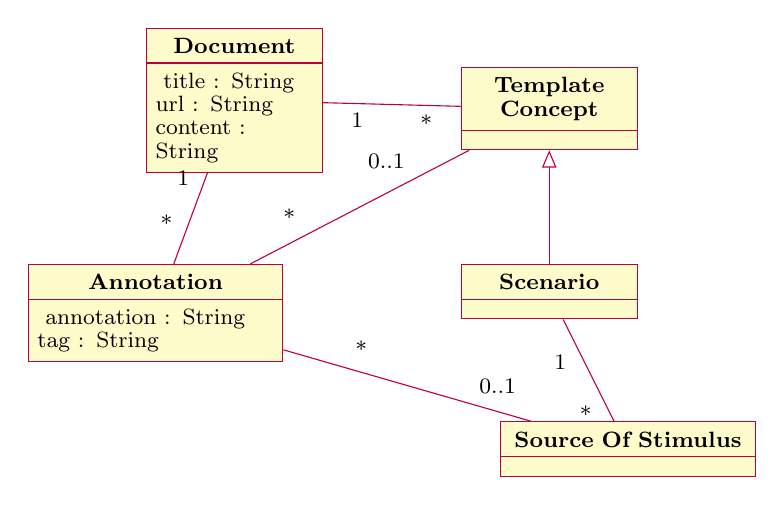
\begin{tikzpicture}
\tikzstyle{every node}=[font=\footnotesize]

\begin{class}[text width=2cm ]{Document}{0,0}
	\attribute { title : String }
	\attribute { url : String }
	\attribute { content : String }
\end{class}

\begin{class}[text width=3cm ]{Annotation}{-1,-3}
	\attribute { annotation : String }
	\attribute { tag : String }
\end{class}

\begin{class}[text width=2cm ]{Template Concept}{4,-0.5}
	\attribute{}
\end{class}

\begin{class}[text width=2cm ]{Scenario}{4,-3}
	\inherit{Template Concept}
	\attribute{}
\end{class}

\begin{class}[text width=3cm ]{Source Of Stimulus}{5,-5}
	\attribute{}
\end{class}

\association{Document}{}{1}{Template Concept}{}{*}
\association{Document}{}{1}{Annotation}{}{*}
\association{Template Concept}{}{0..1}{Annotation}{}{*}
\association{Scenario}{}{1}{Source Of Stimulus}{}{*}
\association{Source Of Stimulus}{}{0..1}{Annotation}{}{*}

\end{tikzpicture}
\caption{Associations between Document, Annotation and the domain model concepts}
\label{figure:documentAnnotationConcepts}
\end{figure}

Annotations are used to enrich the templates described in Section \ref{section:templates}. Associating the annotations with the respective instances of the concepts allows for that enrichment. All the concepts, not only the main ones, can have associated annotations.

As mentioned in the previous section, an annotation can partially or fully describe a concept, therefore a concept can be associated with multiple annotations. 

Figure \ref{figure:documentAnnotationConcepts} shows how the Annotation is associated with the domain concepts. There is an association not only with the main concepts of the domain model, but also all the other concepts represented in \ref{figure:abstractDomainModel}. The figure exemplifies these associations with the Scenario, which is a main concept, and the Source of Stimulus, but all the other concepts and main concepts - all the Scenario Elements, Modules, Components, etc. - have similar associations.  

\subsection{Interface Flow}
\label{section:interfaceFlow}

The associations between the entities described in the previous sections are created after a set of interactions with the system. These interactions are:

\begin{enumerate}
\item After navigation to the document page, a portion of text is selected. The AnnotatorJS interface is prompted, and the user selects a tag to describe the selected text;

\item Upon submission, an instance of ``Annotation'' is created and associated with the instance of the document;

\item By mouse hovering over the highlighted text, another AnnotatorJS interface is prompted, and the user can associate this annotation to a domain entity by clicking ``Add this annotation to the structured representation'';

\item Upon clicking the link, a modal window is shown and, according to the tag given to the annotation, the user can select either an existant Scenario, View or Module to add this annotation to, or create a new instance. 

Initially there are no created instances, and upon creation the instance is associated with the document. When a new Scenario is created, their elements are instantiated as well;

\item After selection, the annotation is associated with the selected element. In the case of Scenarios, if the annotation describes any of the scenario elements, it will be associated with the instance of the corresponding element. 

For example, an annotation tagged as ``Stimulus'' will be associated with the instance of the Stimulus entity that is associated with the selected Scenario.

\item The user is then redirected to the template of the selected element. Inside the template, the user can delete the annotation, move it to other element, delete the element itself and add text descriptions to the template. 

In the Scenario template the user can also add Tactics, in the Module template the user can add relations with other Modules, and in the View template the user can add elements to the view.
\end{enumerate}

Figures \ref{figure:scenarioTemplate2}, \ref{figure:moduleTemplate2} and \ref{figure:viewTemplate2} show the Schemas presented in Section \ref{section:templates} of Chapter \ref{chapter:domainModel}, now including the annotations and the user text.

\begin{figure}
\centering
\lstinputlisting[language=HTML, style=customhtml]{scenarioSchema2.html}
\caption{Scenario Schema enriched with annotations and user text}
\label{figure:scenarioTemplate2}
\end{figure}

\begin{figure}
\centering
\lstinputlisting[language=HTML, style=customhtml]{moduleSchema2.html}
\caption{Module Schema enriched with annotations and user text}
\label{figure:moduleTemplate2}
\end{figure}

\begin{figure}
\centering
\lstinputlisting[language=HTML, style=customhtml]{viewSchema2.html}
\caption{Module Viewtype view Schema enriched with annotations and user text}
\label{figure:viewTemplate2}
\end{figure}

%!TEX root = ../dissertation.tex

\section{Implementation}
\label{implementation}

The application developed follows a Model-View-Controller architecture.

This architecture is composed of three elements \cite{krasner1988description}:
\begin{itemize}
\item The Model, which captures and stores information about the application domain;
\item The View, which generates output based on the model state;
\item The Controller, which provides interaction between the Views and the Model. It is able to modify the Model and update the corresponding View.
\end{itemize}

The standard interaction cycle in this architecture is the following \cite{krasner1988description,reenskaug2009dci}:
\begin{itemize}
\item A user interacting with the application sends a request to the Controller.

\item The Controller communicates with the Model to apply the desired changes.

\item The Model is updated.

\item The Controller notifies the corresponding View so it can be updated with the new version of the Model.
\end{itemize}

The next sections will describe the solution implementation based on these three elements.


\subsection{Model}
\label{section:model}
The Model of the implemented system is based on the Domain Model presented in chapter \ref{chapter:domainModel}, but a few modifications were made to facilitate programming.

The developed application uses the F\'{e}nix Framework, which allows the creation of a transactional and persistent domain model for applications \cite{cachopo2006combining,cachopo2007development}. The domain model is specified in the Domain Modeling Language, which is a domain-specific language created for this framework. The framework completely hides the database from the programmer, who can focus on the application development in Java. 

\subsubsection{Annotations}
\label{subsection:modelAnnotations}
As seen in Chapter \ref{chapter:architecture}, the Document is one of the most important entities, because it aggregates all the annotations created over the text and all the Software Architectures concepts elicited.

Similarly to what is shown in Figure \ref{figure:documentAnnotationConcepts} of Chapter \ref{chapter:architecture}, in the implemented model, the Document entity is connected to the Annotation. However, an annotation is created by an user authenticated in the system, and this information is also present in the domain, as shown in figure \ref{figure:modelDocUserAnnot}. The ``User'' entity saves users registered in the system. When a user creates an annotation, it is associated to him.

\begin{figure}
\centering
\renewcommand {\umltextcolor}{black}
\renewcommand {\umlfillcolor}{none}
\renewcommand {\umldrawcolor}{black}

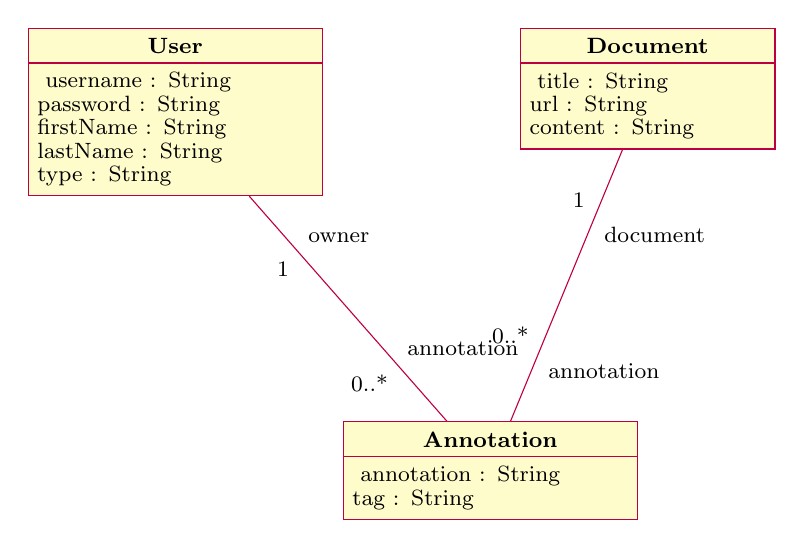
\begin{tikzpicture}
\tikzstyle{every node}=[font=\footnotesize]
\begin{class}[text width=3cm ]{Document}{0,0}
	\attribute { title : String }
	\attribute { url : String }
	\attribute { content : String }
\end{class}

\begin{class}[text width=3.5cm ]{Annotation}{-2,-5}
	\attribute { annotation : String }
	\attribute { tag : String }
\end{class}

\begin{class}[text width=3.5cm ]{User}{-6,0}
	\attribute { username : String }
	\attribute { password : String }
	\attribute { firstName : String }
	\attribute { lastName : String}
	\attribute { type : String}
\end{class}
\association {Document}{document}{1}{Annotation}{annotation}{0..*}
\association {User}{owner}{1}{Annotation}{annotation}{0..*}

\end{tikzpicture}
\caption{Document, Annotations and Users in the implemented Model}
\label{figure:modelDocUserAnnot}
\end{figure} 
 
\subsubsection{Scenarios}
\label{subsection:modelScenarios}
The Scenario is a main concept of the domain, and therefore is connected to the Document, as seen in Figure \ref{figure:documentConcept}. 

Scenarios are represented in the implemented model in a very similar way to what is shown in Figure \ref{figure:abstractDomainModel}. However, there is a difference in the implemented model regarding how Quality Requirements and Tactics are represented.

In Figure \ref{figure:abstractDomainModel}, it is shown an association between Scenario and Quality Requirement, Scenario and Tactic and Tactic and Quality Requirement. The meaning of these associations is to represent what is explained in Section \ref{SAConcepts:Scenarios}: A Scenario has a Quality Requirement from a set of pre-existent ones, and a set of Tactics also from a set of existent ones, which are specific for the Quality Requirement.

However, in the implemented model, there are no pre-existent Tactics nor Quality Requirements. The existent Quality Requirements and their specific Tactics are specified in a Java class, which returns them as necessary. Figure \ref{figure:modelQRTactics} shows the Scenario, Tactic and Quality Requirement entities, and how they are related in the implemented model.

\begin{figure}
\centering
\renewcommand {\umltextcolor}{black}
\renewcommand {\umlfillcolor}{none}
\renewcommand {\umldrawcolor}{black}

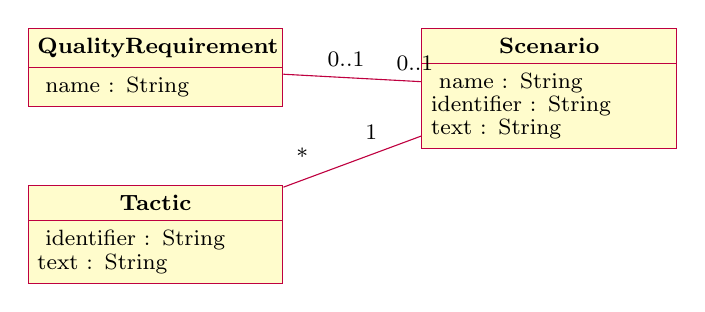
\begin{tikzpicture}
\tikzstyle{every node}=[font=\footnotesize]
\begin{class}[text width=3cm ]{Scenario}{0,0}
	\attribute { name : String}
	\attribute { identifier : String }
	\attribute { text : String }
\end{class}

\begin{class}[text width=3cm ]{QualityRequirement}{-5,0}
	\attribute { name : String}
\end{class}

\begin{class}[text width=3cm ]{Tactic}{-5,-2}
	\attribute { identifier : String }
	\attribute { text : String }
\end{class}

\association {Scenario}{}{1}{Tactic}{}{*}
\association {Scenario}{}{0..1}{QualityRequirement}{}{0..1}

\end{tikzpicture}
\caption{Quality Requirements and Tactics detail in the implemented Model}
\label{figure:modelQRTactics}
\end{figure}

To create a Scenario, it is necessary to select a Quality Requirement from a list, which is retrieved from the class mentioned. When the Scenario is created, a new Quality Requirement is also created, with the selected one stored into the ``name'' attribute, and associated with that Scenario. Tactics can be added once inside the Scenario Template. To add a tactic it is necessary to select it from a list of specific tactics for the quality requirement. That list is, again, retrieved from the class mentioned before. When a specific tactic is selected, a new Tactic is created in the model with the specific tactic name stored in the ``identifier'' attribute. Given these implementation details, there was no need to create the association between Tactic and QualityRequirement nor to have a Quality Requirement associated with many Scenarios.

To facilitate programming, all Scenario elements are a subclass of a ``ScenarioElement'' class, as seen in the example in Figure \ref{figure:modelScenarioElement}. This superclass aggregates all the methods common to the Scenario elements, making it easier to perform actions such as updating the text, associating annotations or presenting the elements in a view. A few of those methods are shown in the figure. However, this class is not associated with the Scenario entity. Its purpose is only to facilitate programming by aggregating common methods. 

\begin{figure}
\centering
\renewcommand {\umltextcolor}{black}
\renewcommand {\umlfillcolor}{none}
\renewcommand {\umldrawcolor}{black}

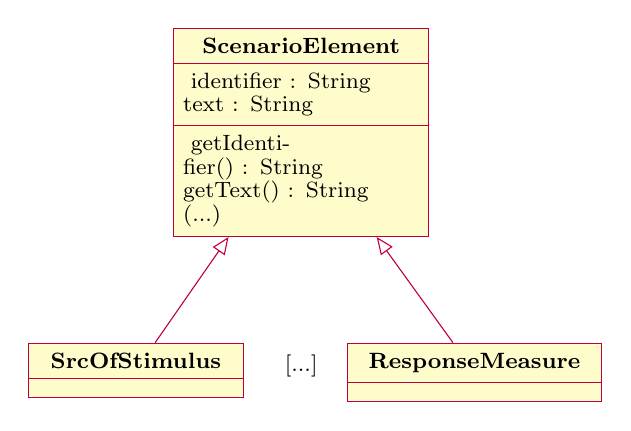
\begin{tikzpicture}
\tikzstyle{every node}=[font=\footnotesize]
\begin{class}[text width=3cm ]{ScenarioElement}{0,0}
	\attribute { identifier : String }
	\attribute { text : String }
	\operation { getIdentifier() : String }
	\operation { getText() : String}
	\operation { (...)}
\end{class}

\begin{class}[text width=2.5cm ]{SrcOfStimulus}{-2.1,-4}
	\inherit{ScenarioElement}
	\attribute{}
\end{class}

\draw [umlcd style] (0,-4.3) node {[...]};

\begin{class}[text width=3cm ]{ResponseMeasure}{2.2,-4}
	\inherit{ScenarioElement}
	\attribute{}
\end{class}		
	
\end{tikzpicture}
\caption{The ScenarioElement entity}
\label{figure:modelScenarioElement}
\end{figure}

The ``identifier'' parameter of the entities, seen in Figures \ref{figure:modelQRTactics} and \ref{figure:modelScenarioElement} stores the name of the concept that corresponds to that entity, and often corresponds to the name of the entity itself. For example, the identifier in all instances of Scenario is ``Scenario'' and the identifier in all instances of ``SrcOfStimulus'' is ``Source Of Stimulus''. This was done to facilitate certain programming issues such as getting the concept name from a ``ScenarioElement'' instance. The ``name'' attribute in the Scenario gives it an identification other than just the quality attribute, and the ``text'' attribute in the Scenario and ScenarioElement corresponds to the description text that can be added to the templates.

All domain entities have associated annotations, as it was mentioned previously in Section \ref{section:annotation}. The implemented model is similar to what is shown in Figure \ref{figure:documentAnnotationConcepts}, with the Scenario and ScenarioElement entities being associated with the Annotation.


\subsubsection{Modules}
\label{subsection:modules}

The Modules are the elements of the Module Viewtype Views. Figure \ref{figure:modelModule} shows how a Module is represented in the implemented model.

\begin{figure}
\centering
\renewcommand {\umltextcolor}{black}
\renewcommand {\umlfillcolor}{none}
\renewcommand {\umldrawcolor}{black}

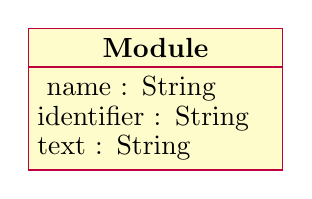
\begin{tikzpicture}
\begin{class}[text width=3cm ]{Module}{0,0}
	\attribute { name : String }	
	\attribute { identifier : String }
	\attribute { text : String }
\end{class}			
\end{tikzpicture}
\caption{The Module entity}
\label{figure:modelModule}
\end{figure}

The Module entity has a ``name'' attribute, which provides identification and also gives an idea on what are the Module functions, an ``identifier'', as explained in the previous section, and a ``text'' attribute, which corresponds to text added to the template.

As it is one of the main concepts of the system, the Module is associated with the corresponding document upon its creation as demonstrated in the example in Figure \ref{figure:documentAnnotationConcepts}. The Module is also associated with the set of Annotations that describe it.

As seen in the abstract domain model present in Figure \ref{figure:abstractDomainModel} of Chapter \ref{chapter:domainModel}, the elements of a view have a certain type of relationship with each others. Although the abstract domain model in Figure \ref{figure:abstractDomainModel} contains an entity ``Relation'' to represent how the view elements are connected, in the case of the Modules, these relations have no other information than the Modules connected. 

Therefore, in the implemented model, there are no entities representing the relationships between modules. Instead, there were defined different associations of the Module entity to itself, in order to represent the different relations.

Each Module Viewtype Style specifies relation types refined from the ones presented in \ref{SAConcepts:Views}. There are, then, eight types of relations between Modules\cite{clements2003documenting} defined in the Domain Modeling Language:
\begin{itemize}
\item \textit{Is-Part-Of} - a Module can be part of one and only one parent Module. Figure \ref{figure:modelIsPartOfRelation} shows how this relation was implemented. A Module can have only one other Module set as parent, but can have many children Modules;
\begin{figure}
\centering
\lstset{style=customjava}
\begin{lstlisting}
relation moduleIsPartOfModule {
	Module playsRole parent{ multiplicity 0..1; }
	
	Module playsRole child{ multiplicity 0..*; }
}
\end{lstlisting}
\caption{Is-Part-Of relation between Modules in the implemented model}
\label{figure:modelIsPartOfRelation}
\end{figure}

\item \textit{Uses} - a specialization of the \textit{depends-on} relation, where a Module depends on the correct functioning of other Modules to satisfy its own requirements. The implementation is shown in Figure \ref{figure:modelUsesRelation}. A Module can use and be used by many other Modules;
\begin{figure}
\lstset{style=customjava}
\begin{lstlisting}
relation moduleUsesModule {
	Module playsRole uses{ multiplicity 0..*; }
	
	Module playsRole usedBy{ multiplicity 0..*; }
}
\end{lstlisting}
\caption{Uses relation between Modules in the implemented model}
\label{figure:modelUsesRelation}
\end{figure}

\item \textit{Is-A} - a relation of generalization, in which a Module is a generalization, similar to a superclass, of other modules. The implementation of this relation is similar to the implementation of the ``Uses'' relation in Figure \ref{figure:modelUsesRelation}, as a Module can be a generalization of many Modules and a specialization of many others (multiple inheritance).

\item \textit{Crosscuts} - an Aspect Module, which implements a crosscutting concern of the system, is bound to a Module that is affected by that crosscutting concern. The Implementation of this relation is similar to the one shown in Figure \ref{figure:modelUsesRelation}, as a Module can be a crosscutting concern of many Modules, and be crosscutted by other Aspect Modules.

\item \textit{One-To-One, One-To-Many, Many-to-Many} - logical associations between Data Entity Modules, similar to the UML associations. The implementation of these relations is, again, similar to the implementation of the ``Uses'' relation in Figure \ref{figure:modelUsesRelation}. The '0..*' cardinality in the one-to-one, one-to-many and many-to-many relations means that a Module can have several relations of this type in a Data Model Style view. For example, if a Module instance with name ``Department'' has a ``One-To-Many'' relation with Modules ``Employee'' and ``Room'', it means that a visual representation of these Modules would be the one in figure \ref{figure:modelOneToManyExample}.
\begin{figure}
\centering
\renewcommand {\umltextcolor}{black}
\renewcommand {\umlfillcolor}{none}
\renewcommand {\umldrawcolor}{black}
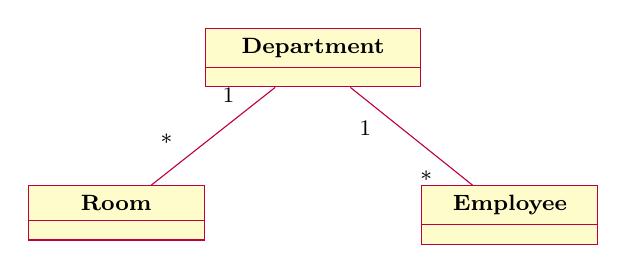
\begin{tikzpicture}
\tikzstyle{every node}=[font=\footnotesize]
\begin{class}[text width=2.5cm ]{Department}{0,0}
	\attribute {}
\end{class}

\begin{class}[text width=2cm ]{Room}{-2.5,-2}
	\attribute {}
\end{class}

\begin{class}[text width=2cm ]{Employee}{2.5,-2}
	\attribute {}
\end{class}

\association{Department}{}{1}{Room}{}{*}
\association{Department}{}{1}{Employee}{}{*}
\end{tikzpicture}
\caption{Example of the One-To-Many relation between Modules}
\label{figure:modelOneToManyExample}
\end{figure}

\item \textit{Aggregation} - an aggregation relation. The implementation of this relation is similar to Figure \ref{figure:modelUsesRelation}, as a Module can be an aggregator of other several Modules, and be aggregated by many others;
\end{itemize}

\subsubsection{Components and Connectors}
\label{subsection:modelComponentsConnectors}
Components and Connectors are the elements of the Component \& Connector Viewtype Views. Figure \ref{figure:modelComponentConnector} shows how these concepts are represented in the implemented model.

\begin{figure}
\centering
\renewcommand {\umltextcolor}{black}
\renewcommand {\umlfillcolor}{none}
\renewcommand {\umldrawcolor}{black}
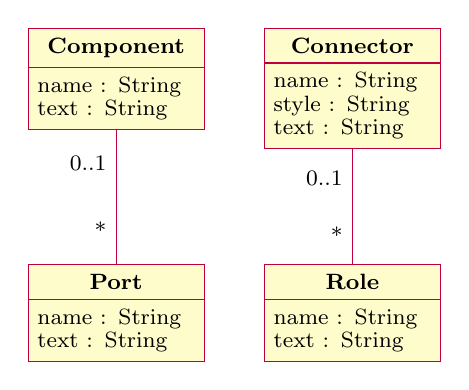
\begin{tikzpicture}
\tikzstyle{every node}=[font=\footnotesize]
\begin{class}[text width=2cm ]{Component}{0,0}
	\attribute {name : String}
	\attribute {text : String}
\end{class}

\begin{class}[text width=2cm ]{Connector}{3,0}
	\attribute {name : String}
	\attribute {style : String}
	\attribute {text : String}
\end{class}

\begin{class}[text width=2cm ]{Port}{0,-3}
	\attribute {name : String}
	\attribute {text : String}
\end{class}

\begin{class}[text width=2cm ]{Role}{3,-3}
	\attribute {name : String}
	\attribute {text : String}
\end{class}

\association{Component}{}{0..1}{Port}{}{*}
\association{Connector}{}{0..1}{Role}{}{*}
\end{tikzpicture}
\caption{Component and Connector entities in the implemented model}
\label{figure:modelComponentConnector}
\end{figure}
 
A Component has a set of Ports, and a Connector as a set of Roles. The Ports of a Component are connected to the Roles of a Connector by the \textit{Attachment} relation explained in Section \ref{domainModel:SAConcepts} of Chapter \ref{chapter:domainModel}. The implementation of this relation will be explained further on. The ``name'' and ``text'' attributes in the entities correspond to the identification name of the entity and the descriptive text that can be added, respectively. The ``style'' attribute in the Connector refers to the Component \& Connector styles. Each style has a unique type of connector. Specifying the style of a connector will make it easier to figure which Components will attach to it.

The Component and Connector are main concepts of the system, and therefore are associated with the corresponding document upon creation. Both the Component and Connector entities and also the Port and Role are associated to a set of Annotations that describe them. The associations of these entities to the Document and Annotation are similar to the ones in the example of Figure \ref{figure:documentAnnotationConcepts}.

Components are related with Connectors by the \textit{Attachment} relation. A Component has, as mentioned, a set of ports, and these ports can be attached to roles of Connectors.

Similar to the Module relations, the \textit{Attachment} relation in the implemented model has no more information than the Port and Role involved. Therefore, it did not make sense to create an entity to represent this relation. Instead, a new relation between the Port and Role entity is created in the Domain Modeling language, as shown in Figure \ref{figure:modelAttachmentRelation}.

\begin{figure}
\lstset{style=customjava}
\begin{lstlisting}
relation portIsAttachedToRole {
	Port playsRole port { multiplicity 0..1; }
	
	Role playsRole role { multiplicity 0..1; }
}
\end{lstlisting}
\caption{Attachment relation between Component Ports and Connector Roles in the implemented model}
\label{figure:modelAttachmentRelation}
\end{figure}


\subsubsection{Views}
\label{subsection:modelViews}

The abstract domain model presented in Figure \ref{figure:abstractDomainModel} of Chapter \ref{chapter:domainModel} shows how a View is related to the Viewtype, the Styles and the elements. 

A View is, as the Scenario, the Element and the Relation, considered a main concept, and therefore has its own dedicated template. Figure \ref{figure:modelView} shows how the View is represented in the implemented model.

\begin{figure}
\centering
\renewcommand {\umltextcolor}{black}
\renewcommand {\umlfillcolor}{none}
\renewcommand {\umldrawcolor}{black}
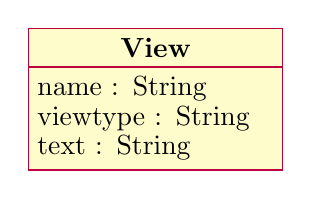
\begin{tikzpicture}
\begin{class}[text width=3cm ]{View}{0,0}
	\attribute {name : String}
	\attribute {viewtype : String}
	\attribute {text : String}
\end{class}
\end{tikzpicture}
\caption{View entity in the implemented model}
\label{figure:modelView}
\end{figure}

In the abstract domain model of Figure \ref{figure:abstractDomainModel} the View is associated with the Viewtype entity which, in turn, is associated with a Style entity. Similar to what was explained for the Scenarios with the Quality Requirements and Tactics, the abstract domain model assumes there are a set of pre-defined Viewtype entities, each associated with a pre-defined set of Styles. 

In the implemented domain model, however, there are no pre-defined Styles nor Viewtypes. When a view is added to the system, a viewtype must be chosen, and it is stored in the ``viewtype'' attribute. This attribute is used to distinguish what kind of elements can be added to the view. For example, if the ``viewtype'' attribute of a View is set to ``Module Viewtype'', then only Modules are added to that View. 

The styles of a view are not explicitly stated, but they are implicit by the elements that are added to the View. For example, a Module Viewtype View containing a set of Modules with ``uses'' relations between each others implies that there is a \textit{Uses} style in the view, and a Component \& Connector Viewtype View containing Components attached to Connectors with a certain style implies that that style is present in the view. This verification is done by the Controller, as described in Subsection \ref{substection:viewController}.

A View is composed by a set of Elements, as seen in Figure \ref{figure:abstractDomainModel}. In the implemented domain model, the View has a similar association with the Module, Component and Connector entities. Figure \ref{figure:modelviewelements} shows how these relations are implemented in the Domain Modeling Language.

\begin{figure}
\lstset{style=customjava}
\begin{lstlisting}
relation viewHasModules {
	View playsRole view { multiplicity 0..*; }
	Module playsRole module { multiplicity 0..*;}
}

relation viewHasComponents {
	Component playsRole component { multiplicity 0..*; }
	View playsRole view { multiplicity 0..*; }
}

relation viewHasConnectors {
	Connector playsRole connector { multiplicity 0..*; }
	View playsRole view { multiplicity 0..*; }
}
\end{lstlisting}
\caption{Relation between View and the view elements: Module, Component and Connector}
\label{figure:modelviewelements}
\end{figure}

A View is created by associating an Annotation with it and, as it is a main concept, it is associated with the respective Document, as demonstrated in the example in Figure \ref{figure:documentAnnotationConcepts}.

\subsection{Controller}

This section describes the Controller part of the implemented system. The application developed uses the Spring\footnote{https://spring.io/} Framework, which allows the definition of one or more Java classes to act as Controllers and handle requests.

A Java class is set to be a Controller by annotating it with the \textit{@Controller} annotation, or \textit{@RestController} if the controller's goal is to provide a REST API. Figure \ref{figure:springController} shows an example from the Document Controller described in \ref{subsection:documentController}, with a method that handles requests for the URL \textit{'/selectDoc/{id}'}. Method \textit{showDocument()} retrieves the Document from the domain model with the specified \textit{id} and adds it and the \textit{id} itself as Model attributes, so the template will be able to use them. The template ``docTemplate'' will be then showed to the user.

\begin{figure}
\lstset{style=customjava}
\begin{lstlisting}
@Controller
public class DocumentController {
	// ...
	@RequestMapping(value = "/selectDoc/{id}", method = RequestMethod.GET)
	public String showDocument(@PathVariable String id, Model m) throws IOException {
		m.addAttribute("docId", id);
		Document d = FenixFramework.getDomainObject(id);
		m.addAttribute("doc", d);
		return "docTemplate";
	}
}	
\end{lstlisting}
\caption{Example of a Controller class defined using the Spring Framework} 
\label{figure:springController}
\end{figure}

\subsubsection{Annotation Controller}
The AnnotationController class provides a way to manage the annotations added to a document. It communicates with the Domain Model to create, remove or update Annotations. This controller is in fact a RestController, which means it provides a REST API, used to retrieve a JSON representation of the annotations stored in the model and display it along with the document text. 
The endpoints provided by this controller are described in Table \ref{table:endpoints}.
	
\begin{table}
\begin{tabular}{ | c | m{1.5cm} | m{3.5cm} |m{7.7cm}|}
    \hline
    \textbf{Name} & \textbf{Request} \textbf{Method }& \textbf{Endpoint} & \textbf{Description}\\ \hline
	INDEX & GET & \parbox[c][1.5cm]{3.5cm}{/selectDoc/\{docId\}/\\store/annotations} & \parbox[c]{8cm}{Returns the set of annotations associated with the \\document with id \textit{docId} }\\ \hline
   	READ & GET & \parbox[c][1.5cm]{3.5cm}{/selectDoc/\{docId\}/\\store/annotations/\{id\}} & Returns the annotation with the specific \textit{id} \\ \hline
    CREATE & POST & \parbox[c]{3.5cm}{/selectDoc/\{docId\}/\\store/annotations} & \parbox[c][1.5cm]{8cm}{Creates a new annotation, stores it in the model \\associated with the document with id \textit{docId}, \\ and redirects to the Read endpoint} \\ \hline
    UPDATE & PUT & \parbox[c][1.5cm]{3.5cm}{/selectDoc/\{docId\}/\\store/annotations/\{id\}} & \parbox[c]{8cm}{Updates the annotation with the given \textit{id} and \\redirects to the READ endpoint} \\ \hline
    DELETE & DELETE & \parbox[t]{3.5cm}{/selectDoc/\{docId\}/\\store/annotations/\{id\}} & \parbox[c][2cm]{8cm}{Removes the association between the \\ annotation with the given id and the document \\ with id \textit{docId}. The response is a HTTP/1.0 204 \\ NO CONTENT.} \\ \hline
  \end{tabular}
  \caption{REST API provided by the Annotation Controller}
  \label{table:endpoints}
\end{table}

The \textbf{INDEX} endpoint has the particularity of iterating through all the Annotations associated with the Document with id \textit{docId}. If the annotation is associated to another domain entity besides the Document (for example, a Scenario, or a Module), information about the domain entity will be added to the annotation body, and will be shown in the interface. This way, it is possible to have some information about the domain entity even before checking its template. 

Figure \ref{figure:annotationControllerIndex} shows an example of how information is added to the annotation in the \textit{INDEX} endpoint. The method \textit{getAnnotations()}, which receives the requests for this endpoint, iterates over the annotations associated with the document with id \textit{docId}, parses the JSON of each annotation into an instance of the AnnotationJS class, checks which domain element is associated with the annotation and adds information accordingly to the field ``text'' of the annotation. The example in the figure shows how information about the viewtype is added to annotations connected with a View. The list of all retrieved AnnotationJS instances is then parsed into a JSON string and sent as response.

\begin{figure}
\lstset{style=customjava}
\begin{lstlisting}
	@RequestMapping(value = "/selectDoc/{docId}/store/annotations", 
	method = RequestMethod.GET)
	
	public String getAnnotations(@PathVariable String docId) {
		Document d = FenixFramework.getDomainObject(docId);
		List<AnnotationJ> anns = new ArrayList<AnnotationJ>();
		Gson g = new Gson();
		for(Annotation a : d.getAnnotationSet()) {
			AnnotationJ ann = g.fromJson(a.getAnnotation(), AnnotationJ.class);
			if(a.isViewAnnotation() && a.getView() != null) {
				View v = a.getView();
				ann.setText("View: " + v.getViewtype());
			}
			//...			
			anns.add(ann);
		}
		String resp = g.toJson(anns);
		return resp;
	}		
\end{lstlisting}
\caption{Example of how the INDEX endpoint adds information to the annotation body}
\label{figure:annotationControllerIndex}
\end{figure}

\subsubsection{Document Controller}
\label{subsection:documentController}
The DocumentController class handles the requests to view, add or remove a document from the system.

Adding and removing documents from the system is a feature that only Teachers are authorized to use. The controller receives a POST request containing the URL to the article. The Java library JSoup\footnote{http://jsoup.org/} extracts the HTML from the given URL and the controller processes it and stores a Document in the database. Processing of the extracted HTML includes turning relative URLs into absolute ones for href and src attributes.
The Controller will also check if the database already contains a document with the given URL before adding a new entry. 

When a teacher removes a Document from the system, all Annotations and Domain Model entities associated with that Document such as Scenarios or Views are removed from the system as well.

Upon Document visualization, there are three other operations handled by this controller:

\begin{itemize}
\item When a user wants to associate an Annotation with a domain entity such as a Scenario, a request is sent to the Document Controller containing information about the annotation unique ID and its tag. Based on the tag, the controller then redirects to another controller, which will provide means for the user to add and/or select an entity to associate with the annotation.

The reason for this redirect is the existent of a logic division of the Controllers. Each Controller class handles a set of requests related with a certain entity of the domain model. The AnnotationController class handles operations over Annotations, the ScenarioController handles operations over Scenarios and their elements, etc. 

Therefore, it's only logical to redirect this request to the Controller that handles operations over the respective domain entity. Figure \ref{figure:documentControllerLinkAnnotation} shows the method in DocumentController that performs the redirect.

\begin{figure}
\lstset{style=customjava}
\begin{lstlisting}
	@RequestMapping(value = "/addAnnotationToStructure/{docId}/{annotationId}/{tag}")
	public RedirectView addAnnotationModal(@PathVariable String docId,
			@PathVariable String annotationId, @PathVariable String tag) {
		RedirectView rv = null;
		if (Utils.allScenarioConcepts().contains(tag)) {
			rv= new RedirectView("/addAnnotationToScenarioStructure/" + docId + "/"
					+ annotationId);
		} else if (tag.contains("Module")) {
			rv = new RedirectView("/addAnnotationToModuleTemplate/" + docId + "/"
					+ annotationId);
		}else if (tag.contains("View")) {
			rv = new RedirectView("/addAnnotationToViewTemplate/" + docId + "/"
					+ annotationId);
		}else if (tag.contains("Component")) {
			rv = new RedirectView("/addAnnotationToComponentTemplate/" + docId + "/"
					+ annotationId);
		}else if (tag.contains("Connector")) {
			rv = new RedirectView("/addAnnotationToConnectorTemplate/" + docId + "/"
					+ annotationId);
		}
		return rv;
	}	
\end{lstlisting}
\caption{Redirecting requests to associate annotations with domain entities in the DocumentController}
\label{figure:documentControllerLinkAnnotation}
\end{figure}

\item When visualizing the Annotation information in the document, it is possible to navigate to the template of the entity to which this annotation is associated by clicking in a link. A request is then sent to the Document Controller, which again checks the Annotation tag, and redirects to the correct Controller. Figure \ref{figure:documentControllerViewTemplate} shows the DocumentController class method which performs the redirect according to the annotation tag.

\begin{figure}
\lstset{style=customjava}
\begin{lstlisting}
	@RequestMapping("/viewTemplate/{docId}/{connectedId}/{annotationId}")
	public RedirectView viewTemplate(@PathVariable String docId,
			@PathVariable String connectedId, @PathVariable String annotationId) {
		Annotation a = FenixFramework.getDomainObject(annotationId);
		RedirectView rv = new RedirectView();
		if(a.isScenarioAnnotation()) {
			rv.setUrl("/viewScenario/"+docId+"/"+connectedId+"#"+annotationId);
		}else if( a.getTag().contains("Module")) {
			rv.setUrl("/viewModule/"+docId+"/"+connectedId+"#"+annotationId);
		}else if(a.getTag().contains("View")) {
			rv.setUrl("/viewView/"+docId+"/"+connectedId+"#"+annotationId);
		}else if(a.getTag().contains("Component")) {
			rv.setUrl("/viewComponent/"+docId+"/"+connectedId+"#"+annotationId);
		}else if(a.getTag().contains("Connector")) {
			rv.setUrl("/viewConnector/"+docId+"/"+connectedId+"#"+annotationId);
		}
		return rv;
	}	
\end{lstlisting}
\caption{Redirecting a request to visualize an entity template in the DocumentController}
\label{figure:documentControllerViewTemplate}
\end{figure}

\item The Document interface also allows the user to navigate to the structured representation of the document, which is an aggregation of all the templates of all the entities added to the system. When the link to navigate to the structured representation is clicked, a request is sent to the Controller, which retrieves information about Scenarios, Views and Elements to be presented to the user. 

Figure \ref{figure:documentControllerStructuredRepresentation} shows the method \textit{viewStructuredRepresentation()}, which handles the request to see the Structured Representation of the Document. This method retrieves all the main elements from the database (scenarios, views, modules, components and connectors) and adds them as model attributes, so they can be used by the template. The template ``structuredRepresentation'' is then returned and showed to the user.

\begin{figure}
\lstset{style=customjava}
\begin{lstlisting}
	@RequestMapping("/viewStructuredRepresentation/{docId}")
	public String viewStructuredRepresentation(@PathVariable String docId,
			Model m) {
		Document d = FenixFramework.getDomainObject(docId);
		m.addAttribute("scenarios", d.getScenarioSet());
		m.addAttribute("views", d.getViewSet());
		m.addAttribute("modules", d.getModuleSet());
		m.addAttribute("components", d.getComponentSet());
		m.addAttribute("connectors", d.getConnectorSet());
		m.addAttribute("docId", docId);
		m.addAttribute("title", d.getTitle());
		return "structuredRepresentation";
	}
\end{lstlisting}
\caption{Retrieving the Structured Representation template in the DocumentController}
\label{figure:documentControllerStructuredRepresentation}
\end{figure}
\end{itemize}

\subsubsection{Scenario Controller}

The Scenario Controller provides means to add and remove Scenarios from the document and link or unlink annotations from a Scenario or its elements.A Scenario is created when a user wants to link an Annotation to a Scenario and is prompted the interface to add a new or choose an existing one. When the Controller receives the request to add a new Scenario, it does not only adds a new Scenario to the database, but also adds a new SrcOfStimulus, Stimulus, Artifact, Environment, Response and ResponseMeasure to the databse, all associated with the newly created Scenario. 

\begin{figure}
\lstset{style=customjava}
\begin{lstlisting}
	@RequestMapping(value = "/addNewScenario/{docId}/{annotationId}/{scenarioName}/
	{qualityRequirement}")
	public RedirectView addNewScenario(/*...*/) {
		addScenarioToDocument(document,qualityRequirement ,scenarioName);		
		//...
	}
		@Atomic(mode = TxMode.WRITE)
	private void addScenarioToDocument(Document d, String qualityRequirement, 
	String scenarioName) {
		Scenario s = new Scenario();
		QualityRequirement qr = new QualityRequirement();
		s.setQualityRequirement(qr);
		//...		
		d.addScenario(s);
	}	
\end{lstlisting}
\caption{Creating a new Scenario in ScenarioController}
\label{figure:scenarioControllerNewScenario}
\end{figure}

Figure \ref{figure:scenarioControllerNewScenario} shows the method \textit{addNewScenario}, which handles the request for adding a new Scenario to the Document and calls the method \textit{addScenarioToDocument()}, which creates the new Scenario with the given name, creates and associates with it the selected Quality Requirement and the Scenario elements and associates it with the respective document.

When the user chooses which Scenario to link the Annotation with, the Controller receives a request containing both the unique ID of the Scenario and the unique ID of the Annotation. With these IDs, it can verify the tag associated with the Annotation, and add the Annotation either to the Scenario or to the corresponding element. 

For example, if the tag associated with the Annotation is ``Source Of Stimulus'', then it will be linked to the ``SrcOfStimulus'' instance that is associated with the Scenario with the specified ID.

Figure \ref{figure:scenarioControllerLinkAnnotation} shows the method \textit{addAnnotationToScenario()}, which associates an Annotation with a Scenario or one of its elements accordingly.

\begin{figure}
\lstset{style=customjava}
\begin{lstlisting}
	@Atomic(mode = TxMode.WRITE)
	private void addAnnotationToScenario(Scenario s, Annotation a) {
		String tag = a.getTag();
		if (tag.equals("Scenario Description") || tag.equals("Tactic")) {
			//associate annotation with the Scenario s
		}
		if (s.getElements().get(tag) != null) {
			//associate annotation with a ScenarioElement
		}
	}	
\end{lstlisting}
\caption{Associating an Annotation with a Scenario in ScenarioController}
\label{figure:scenarioControllerLinkAnnotation}
\end{figure}

A Scenario is initially created without any tactics. These are added in the Scenario Template, and their creation is handled by the Scenario Controller. Upon receiving the corresponding request, a new ``Tactic'' is added to the database containing the tactic's name, and is associated with the corresponding Scenario. When an Annotation with the tag ``Tactic'' is added to a Scenario, it is initially associated with the ``Scenario'' entity, as it can be seen in Figure \ref{figure:scenarioControllerLinkAnnotation}. 

Inside the template, these annotations can be associated with the added tactics. Figure \ref{figure:scenarioControllerLinkToTactic} shows how a request to associate an Annotation with a specific Tactic is handled. In the \textit{linkAnnotationToTactic()} method, the association between the Scenario and the Annotation is removed to create the new association with the Tactic.

\begin{figure}
\lstset{style=customjava}
\begin{lstlisting}
	@RequestMapping(value = "/linkToTactic/{docId}/{scenarioId}/{tacticId}/
		{annotationId}")
	public RedirectView addAnnotationToTactic(/*...*/) {
		//...
		linkAnnotationToTactic(s, t, a);
		//...
	}
\end{lstlisting}
\caption{Associating an Annotation with a specific Tactic in ScenarioController}
\label{figure:scenarioControllerLinkToTactic}
\end{figure}

When user text is added to a Scenario or one of its elements, a request is sent to this Controller. It will then update the Model accordingly and show the updated Model in the corresponding View.

Figure \ref{figure:scenarioControllerText} shows how the Scenario \textit{text} field is updated. The methods for updating the Scenario elements (including Tactics) are very similar to the example in the Figure.

\begin{figure}
\lstset{style=customjava}
\begin{lstlisting}
	@RequestMapping(value = "/setScenarioText/{docId}/{scenarioId}", 
		method = RequestMethod.POST)
	public RedirectView setScenarioText(/*...*/) {
		updateText(scenario, text);
		//...
	}
	
	@Atomic(mode=TxMode.WRITE)
	private void updateText(Scenario scen, String text) {
		scen.setText(text);
	}	
\end{lstlisting}
\caption{Updating the Scenario text in the ScenarioController}
\label{figure:scenarioControllerText}
\end{figure}

\subsubsection{Module Controller}

Similarly to the Scenario Controller, the Module Controller handles the creation and deletion of Modules, which are the elements of Module Viewtype Views. It also handles the linkage of Annotations to existent Modules and the addition of user text to a Module. 

The implementation of the methods that handle these operations is similar to the implementation done in the Scenario Controller. But unlike the Scenario, the Module has no other elements, therefore creating a Module only creates a Module in the database, and annotations are always linked to that Module.

As explained in Chapter \ref{chapter:domainModel}, the Elements of a View are related to each others, and in the Subsection \ref{subsection:modules}, we can see that, since the relations between Modules have no information other than the Modules involved, they are represented in the model as different associations of the ``Module'' entity to itself. 

The Module Controller handles adding and removing other Modules to/from the possible relations. The requests are unique for each relation, meaning the request to add a Module to the \textit{Uses} relation of a certain Module will be in the form \textit{/setModuleUses/...} and the request to add \textit{One-To-One} relations with other Modules to a certain Module will be in the form \textit{/setModuleOneToOne/...}. Each request modifies the corresponding association accordingly.
\begin{figure}
\lstset{style=customjava}
\begin{lstlisting}
	@RequestMapping(value = "/setModuleParent/{docId}/{moduleId}/{parentId}")
	public RedirectView addModuleParent(/*...*/) {
		addParent(module, parent);
		//...
	}
	@Atomic(mode = TxMode.WRITE)
	private void addParent(Module module, Module parent) {
		module.setParent(parent);
	}	
\end{lstlisting}
\caption{Example of adding a ``Is-Part-Of'' relation between two modules}
\label{figure:ModuleControllerIsPartOf}
\end{figure} 

Figure \ref{figure:ModuleControllerIsPartOf} shows how the ModuleController class adds a ``Is-Part-Of'' relation between two modules. Inside a Module template it is possible to select another Module to be the parent and associate them with a ``Is-Part-Of'' relation. The \textit{addModuleParent()} method handles the request to create this association. The request contains the \textit{id} of the module in which the relation will be created, and the \textit{id} of the Module chosen to be the parent. After setting the relation, the user is redirected to the Module template.

\subsubsection{Component and Connector Controllers}

Components and Connectors are the elements of the Component \& Connector Viewtype Views. The ComponentController and ConnectorController classes handle the creation and deletion of Components and Connectors from the system. The two classes have very similar methods.

A Component has a set of Ports, which can be attached to Connector Roles. Adding and removing Ports to a component is very similar to the methods implemented to adding and removing tactics from a Scenario. Initially a Component has no Ports, and these can be created inside the Component template, as shown in Figure \ref{figure:ComponentControllerAddingPorts}. 
\begin{figure}
\lstset{style=customjava}
\begin{lstlisting}
	@RequestMapping(value = "/addPortToComponent/{docId}/{componentId}/{portName}")
	public RedirectView addPortToComponent(/*...*/) {		
		addPortToComponent(component, portName);
		//...
	}

	@Atomic(mode = TxMode.WRITE)
	private void addPortToComponent(Component comp, String portName) {
		Port p = new Port();
		comp.addPort(p);
	}
\end{lstlisting}
\caption{Adding Ports to a Component in ComponentController}
\label{figure:ComponentControllerAddingPorts}
\end{figure}

Annotations with the tag ``Component Port'' are initially associated with the Module, but can be associated with a specific port, as seen in Figure \ref{figure:ComponentControllerLinkToPort}. 

\begin{figure}
\lstset{style=customjava}
\begin{lstlisting}
	@RequestMapping(value = "/moveAnnotationToPort/{docId}/{componentId}/
		{portId}/{annotationId}")
	public RedirectView moveAnnotationToPort(/*...*/) {
		
		moveAnnotationToPort(component, port, annotation);
		//...
	}	
\end{lstlisting}
\caption{Associating an Annotation with a Port in the ComponentController}
\label{figure:ComponentControllerLinkToPort}
\end{figure}

The Connector has a set of Roles, which are attached to the Component Ports. The implementation of the Roles in a Connector is similar to the implementation of the Ports: Initially a Connector has no Roles, which can be added inside the template, and annotations can be associated with the created Roles. The methods for creating Roles and linking annotations to them in the ConnectorController class are very similar to the ones represented in the Figures \ref{figure:ComponentControllerAddingPorts} and \ref{figure:ComponentControllerLinkToPort}, but the requests are sent to \textit{/addRoleToConnector} and \textit{/moveAnnotationToRole/} and instead of Component and Port instances there are Connectors and Roles.

As mentioned in Section \ref{subsection:modelComponentsConnectors}, component ports can be associated with the connector roles by a relation of \textit{attachment}. Inside a Component template, it is possible to attach each of the ports to a Role from an existent Connector.

Figure \ref{figure:ComponentControllerAttachment} shows how an attachment relation is created between a Port and a Role.

\begin{figure}
\lstset{style=customjava}
\begin{lstlisting}
	@RequestMapping(value = "/attachPortToConnectorRole/{docId}/{portId}/{roleId}")
	public RedirectView attachPortToRole(/*...*/) {
		attachPortToRole(port,role);
		//...
	}
	@Atomic(mode=TxMode.WRITE)
	private void attachPortToRole(Port p, Role r) {
		p.setRole(r);
	}
\end{lstlisting}
\caption{Attachment of Component Ports to Connector Roles in the ComponentController}
\label{figure:ComponentControllerAttachment}
\end{figure}

\subsubsection{View Controller}
\label{substection:viewController}

The ViewController class handles the creation and deletion of Views from two possible Viewtypes: Module and Component \& Connector. 

Similar to the other domain entities, a new View is created when the user wants to associate an annotation with the tag ``View'' with a domain entity. Figure \ref{figure:ViewControllerAddModuleViewtype} shows how a request to add a new Module Viewtype View is handled.

\begin{figure}
\lstset{style=customjava}
\begin{lstlisting}
	@RequestMapping(value = "/addNewView/{docId}/{annotationId}/Module Viewtype/{viewName}")
	public RedirectView addNewModuleViewTypeView(/*...*/) {
	
		addModuleViewtypeToDocument(document, viewName, "Module Viewtype");
		//...
	}
\end{lstlisting}
\caption{Adding a new View in the ViewController}
\label{figure:ViewControllerAddModuleViewtype}
\end{figure}

As there are two possible viewtypes for the views added to the application, the ViewController distinguishes between two different templates when receiving a request to view the View's template: One for views from the Module Viewtype, to which only Modules can be added, and one for views from the Component \& Connector Viewtype, to which only Components and Connectors can be added. This distinction is done inside the method \textit{viewViewTemplate()} of the ViewController class. 

Figure \ref{figure:ViewControllerViewTemplates} shows how the method checks the \textit{viewtype} attribute of a View object to add the correct attributes to the template model and return the correct template.
\begin{figure}
\lstset{style=customjava}
\begin{lstlisting}
	@RequestMapping(value = "/viewView/{docId}/{viewId}")
	public String viewViewTemplate(/*...*/) {
		//...
		if(view.getViewtype().equals("Module Viewtype")) {
			m.addAttribute("view", v);
			m.addAttribute("views", d.getViewSet());
			m.addAttribute("modules", d.getModuleSet());
			m.addAttribute("used", new UsedIds());
			return "viewMVTTemplate";
		}else if(v.getViewtype().equals("Component & Connector Viewtype")) {
			//add components and connectors information
		}
		return null;
	}	
\end{lstlisting}
\caption{Request to see a View's Template in the ViewController}
\label{figure:ViewControllerViewTemplates}
\end{figure}
The controller adds the existent Modules, Component and Connectors as template model attributes so the template can show them to the user who wants to add elements to a view. The set of existent Views is also added as attribute, to show in case the user wishes to move an annotation to other view. The UsedIds instance added as attribute is a class containing an empty \textit{List$<$String$>$}, which will be used to save the \textit{ids} of the elements selected to add to a view. 
 
After the user selects a set of Modules, Components or Connectors to add to a view, a request is sent to the ViewController, which handles the association of these elements with the respective view.

Figure \ref{figure:ViewControllerAddModules} shows how Modules are associated with a View, but these methods are similar for the Components and Connectors. 
\begin{figure}
\lstset{style=customjava}
\begin{lstlisting}
	@RequestMapping(value = "/addModulesToView/{docId}/{viewId}", 
		method = RequestMethod.POST)
	public RedirectView addModulesToView(/*...*/@ModelAttribute UsedIds modules) {
		if(view.getViewtype().equals("Module Viewtype")) {
			addModulesToView(v, modules);
		}
		//...
	}
	@Atomic(mode = TxMode.WRITE)
	private void addModulesToView(View v, UsedIds modules) {
		for (String id : modules.getUsed()) {
			//associate module with the view
		}
	}	
\end{lstlisting}
\caption{How Modules are added to a View in ViewController}
\label{figure:ViewControllerAddModules}
\end{figure}
A POST request is sent to \textit{/addModulesToView/\{docId\}/\{viewId\}}, containing in its body the instance of the \textit{UsedIds} class that was added as model attribute (see Figure \ref{figure:ViewControllerViewTemplates}), with the \textit{ids} of the selected elements saved in the list. Method \textit{addModulesToView()} makes sure the view has the correct viewtype for the elements to be added, and then method \textit{addModulesToView(View v, UsedIds modules)} iterates over the list of selected \textit{ids} and associates the Modules with the respective \textit{ids} to the view.

\subsection{Views}
\label{section:Views}
This section describes how the information from the Model is displayed to the user. The developed application uses Thymeleaf\footnote{http://www.thymeleaf.org/}, a Java template engine for displaying dynamic templates. Tymeleaf can be fully integrated with the Spring Framework and, in each template, it is possible to use the its syntax to access and display the Model Attributes added by the Controllers. 

A great advantage of Thymeleaf is the possibility of defining template fragments, which are pieces of code that can be defined in a separate file and be included in any template as desired. One of the main uses of fragments for the developed application is the page header, which is included in all templates and contains a small menu and the logout link. Figure \ref{figure:viewsHeaderFragment} shows how a fragment is defined, in this case with the example of the header. Each fragment must have a unique name, which is ``headerFragment'' in this example. All html code of that fragment is then defined inside the \textit{section} tags.
\begin{figure}
\lstset{style=customhtml}
\begin{lstlisting}
<section layout:fragment="headerFragment">
	<nav class="navbar navbar-inverse" id="headernavbar">
		Header definition here	
	</nav>
</section>
\end{lstlisting}
\caption{Defining the Header fragment in Thymeleaf syntax}
\label{figure:viewsHeaderFragment}
\end{figure}

Including a predefined fragment in a template is as easy as Figure \ref{figure:viewsIncludeFragment} shows. Sending a request to \textit{/headerFragment} will retrieve the whole file where the fragment was defined, and by specifying the fragment name, the html code defined inside \textit{section} tags in the separate files will be included. This means that several fragments can be developed in one single file, and included individually in the templates by specifying their unique name.
\begin{figure}
\lstset{style=customhtml}
\begin{lstlisting}
<section layout:include="@{/headerFragment} :: headerFragment"></section>
\end{lstlisting}
\caption{Including a fragment in Thymeleaf syntax}
\label{figure:viewsIncludeFragment}
\end{figure}

The result of including the header fragment in a template is shown in Figure \ref{figure:viewsHeaderLooks}.

\begin{figure}
\centering
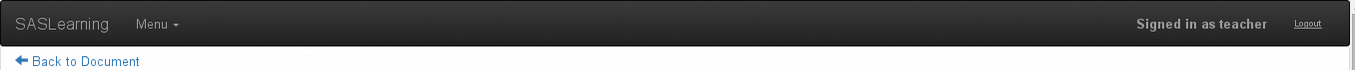
\includegraphics[scale=0.4]{images/header}
\caption{How the header looks when included in a template}
\label{figure:viewsHeaderLooks}
\end{figure}

Another use for this Thymeleaf feature is in the templates defined for the main concepts - View, Scenario, Module, Component and Connector. Each of these templates are defined in separate \textit{$<$section$>$} tags inside a file. This was done because there are other templates where the information about the concepts is included, and it is much easier to include a fragment containing the whole information than writing the code again. 

For example, inside a View template, information about the Elements included in the View must be shown, which is simply a matter of including the template of each element. Other example of the usefulness of these fragments is when showing the structured representation of a document, which consists of showing all the templates of the concepts associated with it. Again, this is as simple as including all the necessary templates.

Figure \ref{figure:viewScenarioTemplate} shows the Scenario template.
\begin{figure}
\centering
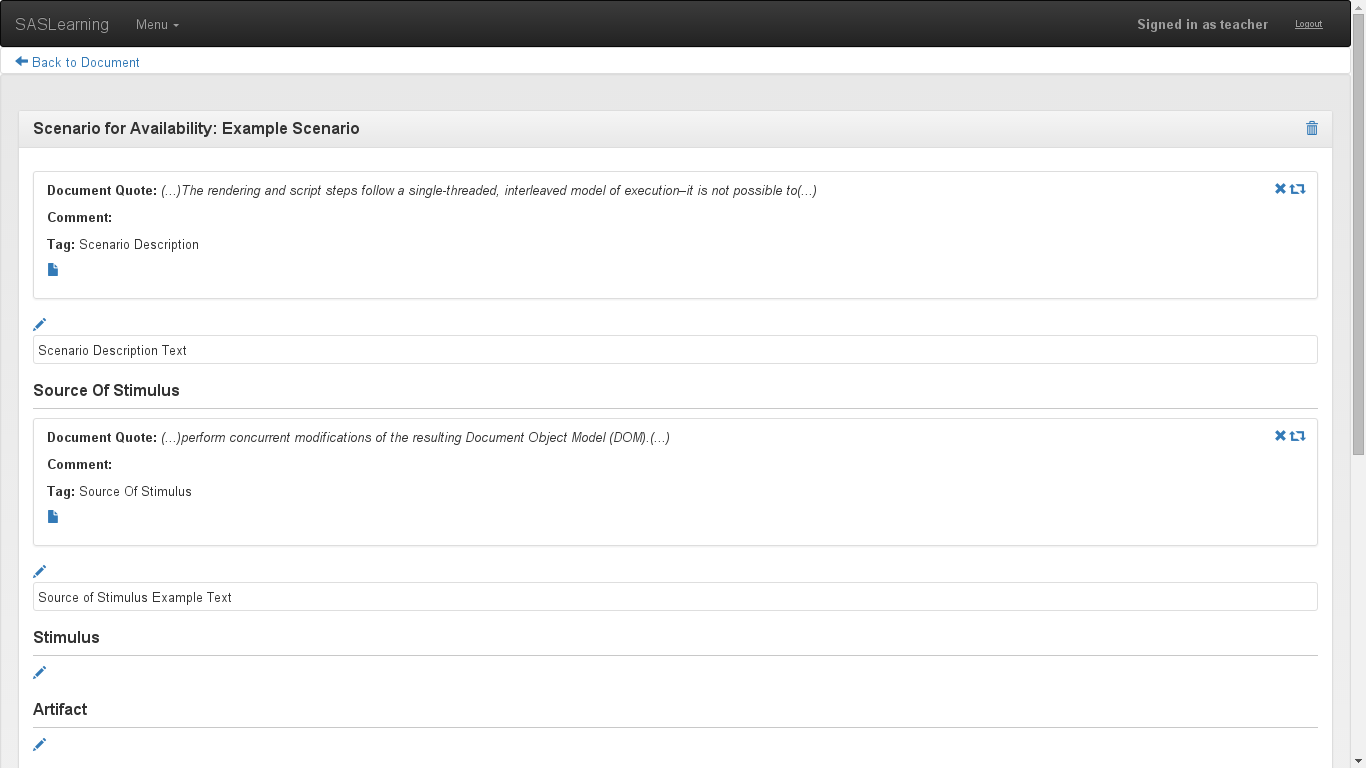
\includegraphics[scale=0.3]{images/scenarioExample}
\caption{Example of the Scenario Template}
\label{figure:viewScenarioTemplate}
\end{figure}
The templates use the information added by the Controllers to the Model Attributes, as seen in Figure \ref{figure:documentControllerStructuredRepresentation} and display it in a structured way. The information added by the Controllers is actually Java objects retrieved from the Model. Thymeleaf allows to treat these attributes as Java objects, so it is possible to obtain the value of the class attributes, or call methods on that object. 

For example, to obtain the Scenario title including the Quality Requirement and the Scenario name as it can be seen in Figure \ref{figure:viewScenarioTemplate}, it is used the Thymeleaf syntax seen in Figure \ref{figure:viewsCallingMethods}. The \textit{\$\{\}} syntax allows to access the variables, and the \textit{th:text} attribute is in fact a Thymeleaf attribute which will set the text inside the \textit{span} tag to the result of the variable access done inside the quotes. As it shown, it is also possible to concatenate the values returned with other static text to obtain the desired results.
\begin{figure}
\lstset{style=customhtml}
\begin{lstlisting}
<span th:text="'Scenario for '+${scenario.getQualityRequirement().getName()}+': '">
</span> 
<span th:text="${scenario.getName()}"></span>
\end{lstlisting}
\caption{How Thymeleaf accesses variables}
\label{figure:viewsCallingMethods}
\end{figure}

Thymeleaf also provides automatic binding of forms information to provided objects. For example, when a user wants to add Modules to a Module Viewtype View, a modal window is prompted, listing all the existent Modules associated with the respective Document, as it is shown in Figure \ref{figure:viewsModalFormExample}. The Modules are listed inside a form, with checkboxes that allow the user to select more than one Module to add. 

\begin{figure}
\centering
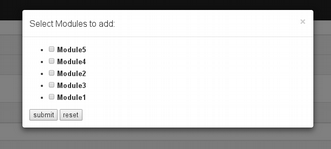
\includegraphics{images/modalExample}
\caption{Example of a Modal window containing a form}
\label{figure:viewsModalFormExample}
\end{figure}

In Figure \ref{figure:ViewControllerViewTemplates}, it is possible to see that the Controller creates and adds a new instance of the \textit{UsedIds} as a model attribute. This instance is used by Thymeleaf to bind the value of the selected checkboxes in the form to the \textit{List$<$String$>$} attribute of the class. Figure \ref{figure:viewFormBindingResult} shows how the form is created.
\begin{figure}
\lstset{style=customhtml}
\begin{lstlisting}
<form action="#" th:action="@{/addModulesToView/}" method="post">
	<ul>
		<li th:each="module : ${modules}" th:object="${used}">
			<input type="checkbox" th:field="*{used}" 
				th:value="${module.getExternalId()}"></input>
			<label th:text="${module.getName()}"></label>
		</li>
	</ul>
</form>
\end{lstlisting}
\caption{Example of a form with object for binding results}
\label{figure:viewFormBindingResult}
\end{figure}
A checkbox is added for each Module in the set. The \textit{th:object} attribute defines that the variable ``used'' is the object to which the results will be bound, and the \textit{th:field} attribute in the \textit{input} tag defines that the value of the checkbox, defined by the \textit{th:value} attribute, if it is chosen, must be bound to the field ``used'' of the class ``UsedIds'', which is the list of type String.

When the form is submitted, Thymeleaf will add the selected values to the list, and send the object in the body of the POST request to the Controller, which will process them as seen in Figure \ref{figure:ViewControllerAddModules}.

%!TEX root = ../dissertation.tex

\section{Evaluation}
\label{evaluation}

The success of a software system is often dependent on the opinion of the people that will use it. Systems attractive and easy to use according to the target audience background are more likely to be highly used.

The developed system tries to make the task of reading, understanding and structuring a software description article into an easy one, providing a simple and clean interface.

As the main goal of the developed application is to be used by students and teachers, in both classroom and home environments, it was asked to the students enrolled in the Software Architectures course to test the application, namely the features for annotating text and structuring Scenarios from the annotations created.

The participating students were asked to fill a small survey afterwards to register their opinions.
This survey consisted of two questions asking to evaluate the Usability and the adequacy of the application regarding Scenario creation in a scale of one to ten, and three open and optional questions, asking what did the student like the most about the application, what improvements could be done to it, and to register any other feedback the student may had.

A total of [NUMBER] students tested and evaluated the application. 

Regarding the usability of the application, Figure ... shows the graph containing the ratings given by the students.

Conclusions....

Regarding the adequacy of the application to create Scenarios, Figure ... shows the graph with the ratings given by the students.

Conclusions...
\begin{figure}
\centering
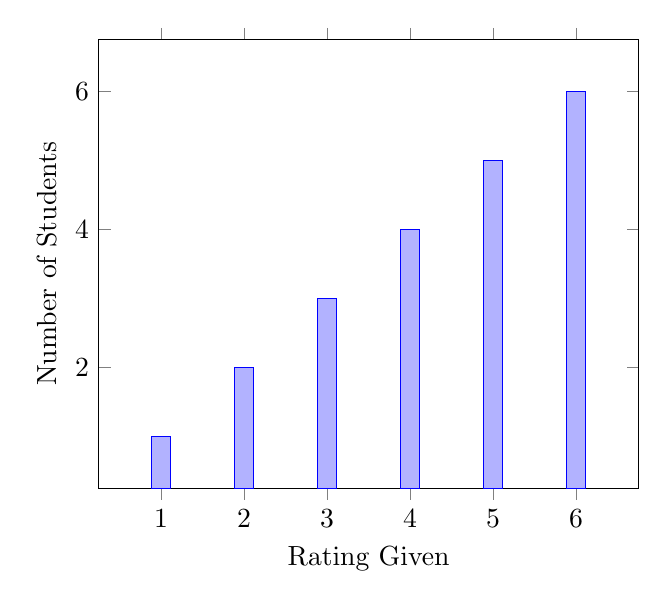
\begin{tikzpicture}
\begin{axis}[
colormap/blackwhite,
x tick label style={
/pgf/number format/1000 sep=},
ylabel=Number of Students,
xlabel=Rating Given,
enlargelimits=0.15,
legend style={at={(0.5,-0.15)},
anchor=north,legend columns=-1},
ybar,
bar width=7pt,
]
\addplot 
	coordinates {(1,1) (2,2) 
		(3,3) (4,4) (5,5) (6,6)};
\end{axis}
\end{tikzpicture}
\end{figure}

Regarding the open questions... Introduzir conclusoes se as houver.
 
%!TEX root = ../dissertation.tex

\section{Future Work}
\label{futureWork}

The analysis of the state-of-the-art on Social Software and Knowledge Structuring done in Chapter \ref{chapter:relatedwork} elicits a set of features that should be present in the solution.

However, developing a platform that provides structuring knowledge from an unstructured source and all the described social features was a very ambitious goal for the time span available. 

The most important feature for this platform was, in fact, the knowledge structuring part, as the main goal of this thesis is to provide a solution to facilitate the analysis of the software description article and help the students to find the correlation between the concepts learned in the theoretical classes and these articles analyzed in the practical ones.

Therefore, the developed solution focused on the association of tags from a closed vocabulary to parts of text, and the creation of a semi-structured representation of the software description articles, where the elements of the Software Architectures are clearly distinguished and described by the corresponding parts of text and user text.

Finding the correct way to make these associations and representations was not a easy task, and there are still details of the developed solution that could be improved and new features that could be added in the future.

\subsection{Allocation Viewtype}

The Module and Component \& Connector Viewtypes are the most common views present in a software description article, and were the ones that got most attention during development.

Allocation viewtype elements should be added to the platform in a future version, so Allocation Viewtype Views can be added to the structured representation of the article.

\subsection{Graphical Representation of Views}

The developed solution allows for the creation and representation of Modules, Components, Connectors and the Views that include these elements. 

Module and Component \& Connector Viewtypes are only represented textually in the platform. However, a good way to represent these views so that the relations between the elements are visible is to represent them in graphical diagrams. 

Features to create or upload graphical representations of Views would be very useful for the platform as a way to improve comprehension about the Views and their elements.

\subsection{Social Elements}

Sections \ref{section:relatedWorkHoneycomb}, \ref{section:relatedWorkPersuasive} and  \ref{section:relatedWorkRepSys} of Chapter \ref{chapter:relatedwork} describing the Related Work list a series of social features that could be useful in the platform.

The developed platform contains social elements and allows for collaboration, as students are individually identified within the system and work together over a shared article. However, there are several other social software elements that could enrich the platform as a social system:

\begin{itemize}
\item \textbf{Groups:} This is the most important social aspect that could be added to the platform, as besides reading and analyzing articles in the practical classes, students must also read and analyze other articles for Group Assignments. The existence of features for the registration of work groups and having articles with group-access only could make it easier for the students to work on their group assignments.

\item \textbf{Q\&A and/or Discussion Forums:} It may not always be clear for a student which parts of the text correspond to which concepts. Although they can simply ask the teacher or a colleague, it could also be very useful to have a central place to ask questions and discuss decisions. Having a discussion forum and/or a Q\&A system could also improve collaboration between students.

\item \textbf{Reputation System: } Although its role would only be motivational, it is important that students feel motivated to participate in the platform, and a reputation system, assigning scores to, for example, annotations or comments, could be useful in this platform.

\item \textbf{Spotlight: } Having a spotlight of the students with most participations and/or the highest reputation scores would provide not only extra motivation, but also promote some healthy competition between students.
\end{itemize}


\section{Conclusions}

In the context of the Software Architectures course, relating theory concepts with descriptions of real systems is a very hard job, specially for students that are learning these concepts for the first time. It is clear that a way for students to discuss and collaboratively structure their knowledge is needed.

This document presents the state-of-the-art on Social Software and Knowledge Structuring: The Honeycomb Framework for social software, design patterns for persuasive software, the roles of users in social software, reputation systems, collaborative tagging, semi-structured contents and ontology learning.

Based on the state-of-the-art presented and the context of the Software Architectures course, this document presents an architecture for a collaborative platform where students can create a structure to relate the theory concepts with the text from systems descriptions.

The main goal for this work is to develop the platform with the knowledge structuring elements and discussion methods, to allow students to discuss and organize thoughts. Additionally, other social software elements will be added, such as reputation systems, in order to boost motivation and encourage participation. 

%
% ---- Bibliography ----
%
\bibliography{mybib}
\bibliographystyle{plain}
\end{document}
